%%%%%%%%%%%%%%%%%%%%%%%%%%%%%%%%%%%%%%%%%
% Short Sectioned Assignment
% LaTeX Template
% Version 1.0 (5/5/12)
%
% This template has been downloaded from:
% http://www.LaTeXTemplates.com
%
% Original author:
% Frits Wenneker (http://www.howtotex.com)
%
% License:
% CC BY-NC-SA 3.0 (http://creativecommons.org/licenses/by-nc-sa/3.0/)
%
%%%%%%%%%%%%%%%%%%%%%%%%%%%%%%%%%%%%%%%%%

%----------------------------------------------------------------------------------------
%	PACKAGES AND OTHER DOCUMENT CONFIGURATIONS
%----------------------------------------------------------------------------------------

\documentclass[paper=a4, fontsize=11pt]{scrartcl} % A4 paper and 11pt font size

\usepackage[T1]{fontenc} % Use 8-bit encoding that has 256 glyphs
\usepackage{fourier} % Use the Adobe Utopia font for the document - comment this line to return to the LaTeX default
\usepackage[brazil]{babel} % Brazil language/hyphenation
\usepackage{graphicx}			% Inclusão de gráficos
\usepackage[utf8]{inputenc}		% Cod. do doc. (conversão auto. dos acentos)
\usepackage{verbatim}     % comentario de varias linhas

\usepackage{amsmath,amsfonts,amsthm} % Math packages

%\usepackage{lipsum} % Used for inserting dummy 'Lorem ipsum' text into the template
\usepackage{float}


\usepackage{sectsty} % Allows customizing section commands
\allsectionsfont{\centering \normalfont\scshape} % Make all sections centered, the default font and small caps

\usepackage{fancyhdr} % Custom headers and footers
\pagestyle{fancyplain} % Makes all pages in the document conform to the custom headers and footers
\fancyhead{} % No page header - if you want one, create it in the same way as the footers below
\fancyfoot[L]{} % Empty left footer
\fancyfoot[C]{} % Empty center footer
\fancyfoot[R]{\thepage} % Page numbering for right footer
\renewcommand{\headrulewidth}{0pt} % Remove header underlines
\renewcommand{\footrulewidth}{0pt} % Remove footer underlines
\setlength{\headheight}{13.6pt} % Customize the height of the header

\numberwithin{equation}{section} % Number equations within sections (i.e. 1.1, 1.2, 2.1, 2.2 instead of 1, 2, 3, 4)
\numberwithin{figure}{section} % Number figures within sections (i.e. 1.1, 1.2, 2.1, 2.2 instead of 1, 2, 3, 4)
\numberwithin{table}{section} % Number tables within sections (i.e. 1.1, 1.2, 2.1, 2.2 instead of 1, 2, 3, 4)

\setlength\parindent{0pt} % Removes all indentation from paragraphs - comment this line for an assignment with lots of text

%----------------------------------------------------------------------------------------
%	TITLE SECTION
%----------------------------------------------------------------------------------------

\newcommand{\horrule}[1]{\rule{\linewidth}{#1}} % Create horizontal rule command with 1 argument of height

\title{	
\normalfont \normalsize 
\textsc{Raul Hacker Club} \\ [25pt] % Your university, school and/or department name(s)
\horrule{0.5pt} \\[0.4cm] % Thin top horizontal rule
\huge Tutorial Primo  \\ % The assignment title
\horrule{2pt} \\[0.5cm] % Thick bottom horizontal rule
}

%\author{} % Your name

\date{\normalsize\today} % Today's date or a custom date

\begin{document}

\maketitle % Print the title

%---------------------------------------------------------------------------------------
%		Espaçamentos entre parágrafos
\setlength{\parindent}{1.3cm}  % Tamanho do parágrafo
\setlength{\parskip}{0.2cm}  % espaçamento entre os parágrafos 


%----------------------------------------------------------------------------------------
%	Primeira seção
%----------------------------------------------------------------------------------------

\textbf{NOTA DO DOCUMENTO}: Este documento foi compilado por Pedro Alcantara, Manoelito Filho e Felipe Bomfim a partir do github do projeto Primo (https://github.com/primo-io/). O intuito desse trabalho é disponibilizar, em forma de documento, as instruções fornecidas nesses repositórios, afim de aumentar a acessibilidade da informação para todos. As traduções e imagens foram retiradas do repositório (\textit{prototype-documentation}). Este documento esta sob a licença CC by-nc-sa-3.0.

\section{O que é o Primo?}

\begin{figure}[H] % Poderia ser \begin{figure}[posicionamento], onde o posicionamento pode ser h - no local do texto onde foi  o comando, t - no topo da pagina atual ou b - no final da pagina de trabalho.
\centering
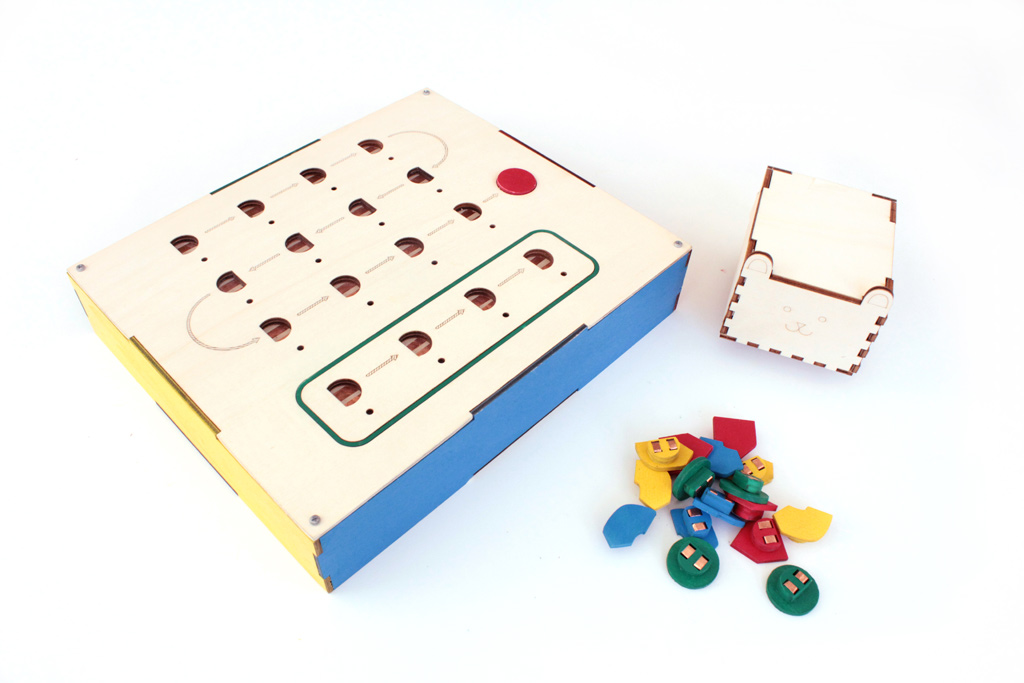
\includegraphics[scale=0.35]{./imagens/primo.jpg}
\caption[ ]{Primo}
%\label{fig:obstaculos}
\end{figure}

Primo é uma interface física projetada para introduzir a lógica de programação para crianças pequenas (de 3 a 7 anos), sem a necessidade de alfabetização. O objetivo do jogo é conduzir um pequeno robô, chamado Cubetto, de volta para sua casa. Para alcançar o objetivo, as crianças devem programar o robô usando um conjunto limitado de instruções: em frente, à esquerda, à direita e função. Enquanto as primeiras três instruções são bem intuitivas, essa última chama uma sub-rotina, uma linha extra de instruções empacotadas em um único comando.

%----------------------------------------------------------------------------------------
%	Segunda seção
%----------------------------------------------------------------------------------------
\section{Pesquisa}

O ensino de programação para crianças é um campo já amplamente debatido. Nós já conhecemos algumas soluções que possuem esse mesmo objetivo, mas para crianças acima de 8 anos. Entretanto, não existem muitas soluções adaptadas para crianças mais novas e não existe nenhuma que trabalha sem a necessidade de telas e de pré-alfabetização. Vemos um número crescente de aplicativos para \textit{tablets} e computadores que também trabalham em conjunto com robôs, mas nenhum deles é completamente livre do domínio do pixel como é o nosso conjunto Primo.

A madeira foi escolhida como o material principal, em primeiro lugar, porque é natural; traz uma sensação mais 'quente' e tem uma sonoridade bacana. A segunda razão é cultural. Foram realizadas pesquisas sobre brinquedos utilizados em jardins de infância tradicionais na Suíça (onde o produto foi originalmente concebido) e foi descoberto que os jogos mais queridos pelas crianças eram aqueles feito com madeira. Brinquedos de madeira são, de maneira geral, muito duráveis e você pode ver as marcas e arranhões neles, sinais de seu uso por outras crianças. É um material com memória. A madeira foi escolhida também como material por conta do forte contraste que ela cria com o uso da tecnologia. Dentro do Primo existe um circuito integrado, mas nós queríamos criar uma experiência 'mágica', escondendo propositadamente a complexidade existente no conjunto.

\begin{figure}[h] % Poderia ser \begin{figure}[posicionamento], onde o posicionamento pode ser h - no local do texto onde foi  o comando, t - no topo da pagina atual ou b - no final da pagina de trabalho.
\centering
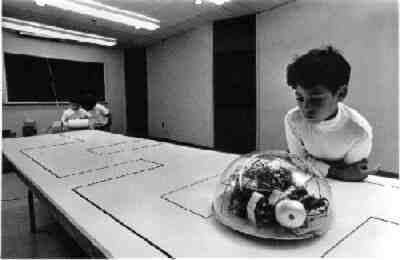
\includegraphics[scale=0.35]{./imagens/logo-turtle.jpg}
\caption[logo_t ]{Logo\_turtle}
%\label{fig:obstaculos}
\end{figure}

O conceito por detrás do Primo é muito inspirado pelo trabalho de Seymour Papert, um matemático que foi o co-fundador do Laboratório de Inteligência Artificial no MIT, juntamente com Marvin Minsky nos anos sessenta (se você está interessado nesse tema, sugerimos que você leia \textbf{pesquisar nome do livro} seu livro mais famoso).Ele dirigia a equipe que inventou o \textbf{LOGO} \textit{(http://en.wikipedia.org/wiki/Logo(programming language)}, provavelmente o recurso mais amplamente utilizado para o ensino de programação para crianças. O objetivo de Seymour Papert não era apenas ensinar a programar, mas também ajudar as crianças a descobrir a sua maneira pessoal de resolver problemas. Primo pode ser considerado uma grande simplificação do LOGO e da 'tartaruga', que era a sua interface física. Nós limitamos as nossas instruções à sua mais pura forma, evitando qualquer tipo de linguagem numérica ou textual.

O primeiro protótipo do Primo foi realizado no SUPSI Lugano, por Matteo Loglio (co-fundador do Primo e designer de interação), durante o (\textbf{MAInD - Master of Advanced Studies in Interaction Design}).A formação de Matteo é em design do produto e depois de aprender o básico sobre Arduino e sua programação, suficientes para a criação do protótipo, ele começou a procurar por soluções técnicas que eram acessíveis para um novato, com o intuito de desenvolver um produto como o Primo. Existiam dois problemas principais: a execução de um carro-robô desde o zero e uma interface que pudesse reconhecer facilmente diferentes instruções.

O primeiro problema foi resolvido com o uso de uma placa (\textbf{Oh\_Oh board, link fora do ar}) de  David Cuartielles, um dos fundadores do Arduino, que havia dado uma palestra no SUPSI. O Oh\_Oh robot é um projeto Open Source - de código aberto - e você pode acessar os arquivos fonte no link acima. É basicamente um Arduino em forma de carro, apenas com um Xbee adicionado para a comunicação via radio.

A segunda questão era projetar uma maneira confiável de detectar os blocos de instrução. A solução foi inspirada por um projeto chamado ["Barcode Piano"].

A idéia era usar blocos bem simples, que poderiam ser reconhecidos pela placa usando resistores. É uma operação básica de divisão de voltagem, com os pinos analógicos do Arduino lendo os valores dos resistores. É um método bem simples mas bastante eficiente para um protótipo.

No campo do design, algumas características ainda precisavam ser testadas; o design atual é o resultado de muitas iterações.

O a escolha do formato de 'cobra' ou ‘zig-zag' para a sequência de instruções foi escolhida para evitar pré-concepções relacionadas com a alfabetização.  

\begin{figure}[htb] % Poderia ser \begin{figure}[posicionamento], onde o posicionamento pode ser h - no local do texto onde foi  o comando, t - no topo da pagina atual ou b - no final da pagina de trabalho.
\centering
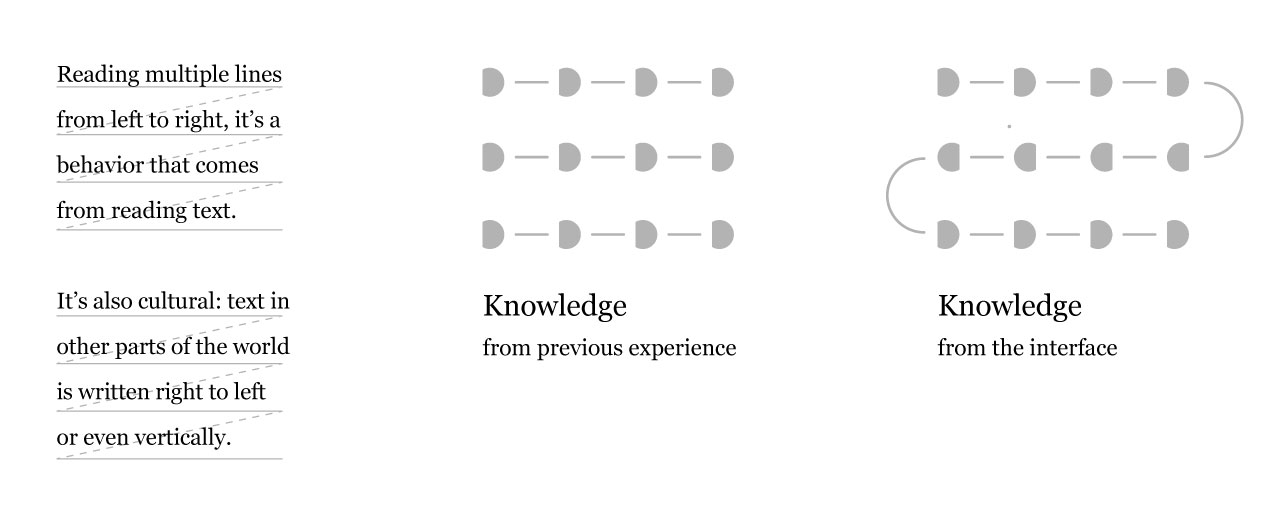
\includegraphics[scale=0.25]{./imagens/left-to-right.jpg}
\caption[ ]{Forma de organização dos blocos de instruções na interface}
%\label{fig:obstaculos}
\end{figure}

 
 O formato em 'D' dos blocos conectores foi projetado para que os mesmos pudessem ser inseridos de uma só maneira, sendo consistentes com o desenho do caminho e com a direção a ser seguida pelo carro. Múltiplos designs poderiam ser usados para isso. O formato em D foi escolhido pois é basicamente 'um circulo com orientação' e também porque de certa maneira remete a um quadro de avisos, um objeto familiar.
 
 
 \begin{figure}[t] % Poderia ser \begin{figure}[posicionamento], onde o posicionamento pode ser h - no local do texto onde foi  o comando, t - no topo da pagina atual ou b - no final da pagina de trabalho.
 \centering
 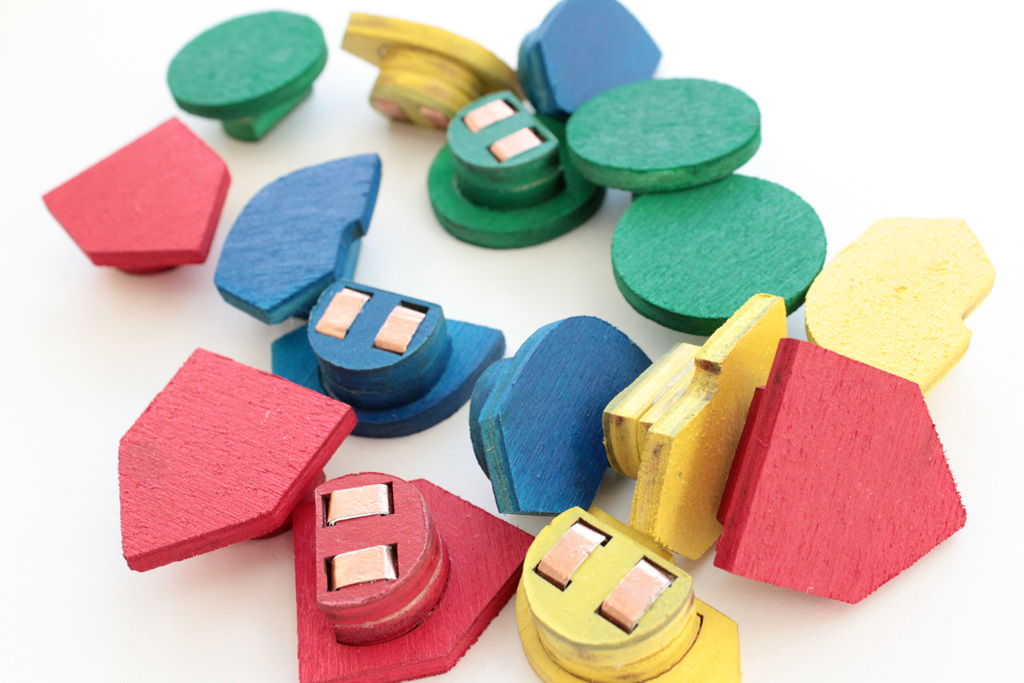
\includegraphics[scale=0.15]{./imagens/instruction-blocks.jpg}
 \caption[ ]{Blocos de instruções}
 %\label{fig:obstaculos}
 \end{figure}
 
 O desenho do formato dos blocos de instrução ainda está sendo testado. O design atual funciona bem, as crianças pegam facilmente o significado. Eles apenas tem alguma dificuldade inicial para se familiarizarem com os blocos de comando ‘direita' e ‘esquerda’. Isso ocorre também porque, em geral, esses conceitos de direção também são novos para os pequenos. Continuamos testando outros formatos de blocos para aprimorar ainda mais essa questão.
 
 No início, o robô tinha a forma de um carrinho de brinquedo e era uma forma bem complicada, que consumia um tempo enorme para ser produzida, pois era toda cortada à laser, colada camada por camada e depois lixada por mais de uma hora. O carro também continha um outro problema, que era ser muito orientado para meninos. Queríamos evitar a discussão com os produtores de brinquedos educativos e sermos criticados por fazermos apenas brinquedos para meninos. Queríamos nos manter neutros e não criar um brinquedo específico para meninos ou meninas, então optamos por uma geometria super neutra, uma caixa.
 
  
  \begin{figure}[h] % Poderia ser \begin{figure}[posicionamento], onde o posicionamento pode ser h - no local do texto onde foi  o comando, t - no topo da pagina atual ou b - no final da pagina de trabalho.
   \centering
   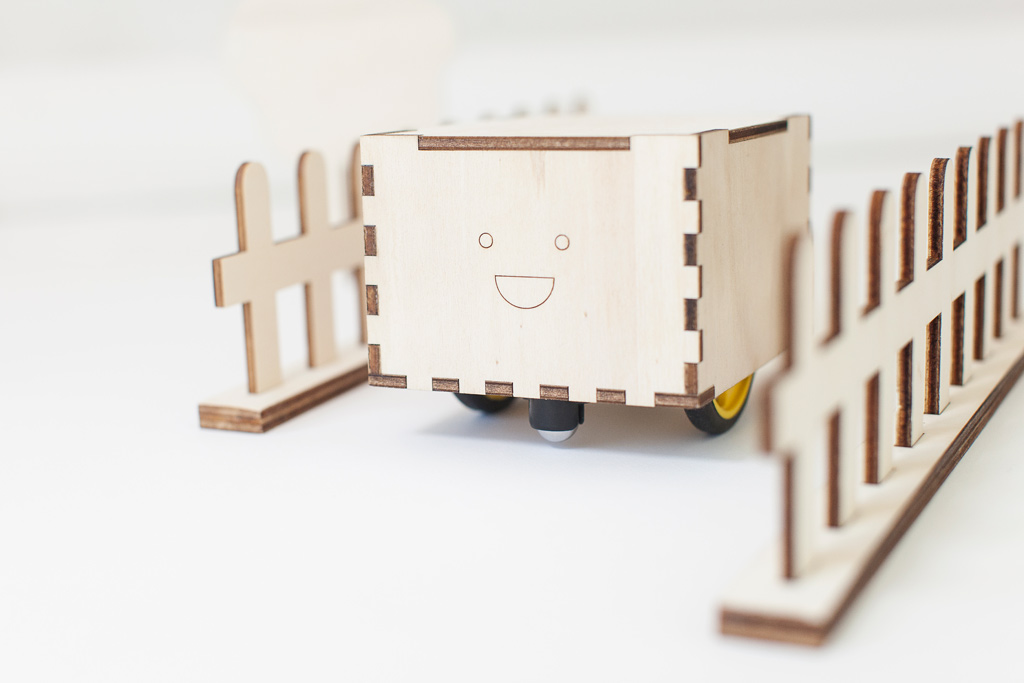
\includegraphics[scale=0.15]{./imagens/cubetto.jpg}
   \caption[ ]{Cubetto}
   %\label{fig:obstaculos}
   \end{figure}
 
 Demos um nome para a caixinha, junto com uma carinha sorridente, fazendo-o mais chamativo para as crianças. O robô foi chamado de Cubetto (cubinho em italiano). A idéia com o Cubetto é também criar um módulo básico que pode ser expandido e customizado facilmente no futuro.

  
   
%-----------------------------------------------------------
%   Terceira seçao
%-------------------------------------------------
\section{Começando}
\subsection{O básico}

Primo é composto por três partes: a Mesa de Interface, o Cubetto e um conjunto de Blocos de Instrução. As crianças interagem com a Mesa colocando os Blocos de Instrução nos orifícios para criar uma seqüência (Um programa) que o Cubetto vai executar.

Existem quatro tipos de Blocos de Instrução, o que significa que resistores com 4 valores distintos podem ser usados, preferencialmente com valores distantes uns dos outros.

Os Blocos são inseridos nos orifícios da Mesa de Interface, onde o valor do resistor é identificado. Depois disso, os valores são processados em uma ‘fila’, que é enviada ao Cubetto usando dois módulos Xbee. Então o Cubetto executa as instruções, uma após a outra.

O cérebro do protótipo é feito com duas placas Arduino, uma UNO (uma Leonardo ou uma Duemilanove também funcionam) para o Cubetto e uma Mega para a Mesa de Interface, onde são necessárias 16 entradas analógicas.

\subsection{Eletrônica}
\subsubsection*{Ferramentas Necessárias}

\begin{itemize}
\item Ferro de solda
\item Solda
\item Fios
\item Pistola de cola quente
\item Cola de madeira
\item Fita de cobre com 5mm de largura

\end{itemize}

\subsubsection*{Componentes}

\textbf{CUBETTO}
\begin{itemize}
\item Arduino UNO (ou Leonardo) 
\item Módulo Arduino Proto Wireless Shield 
\item Driver para Motor SN754410 
\item XBee (série 1 ou 2, não faz diferença) 
\item Rodas SolarBotics  x 2 
\item Motores GM3 SolarBotics x 2 
\item 2 rodizios de metal 
\item Interruptor óptico refletivo CNY70 x 2 
\item (opcional) Suporte de bateria 
\item (opcional) 4 x Baterias recarregáveis
\end{itemize}
 
\

\textbf{MESA DE INTERFACE}


\begin{itemize}
\item Arduino Mega 2560
\item Módulo Arduino Proto Wireless Shield 
\item XBee (série 1 ou 2, não faz diferença) 
\item 16 LEDs 5mm Vermelho
\item 16 Resistores 220 $\Omega$
\item 16 Resistores 10K $\Omega$ 
\item 1 Chave tipo Push Button NA sem trava
\item 50 Conectores macho simple
\item 16 Conectores macho duplos
\item 50 Conectores fêmea
\item 16 Imãs ø 4 h 3
\end{itemize} 

\

\textbf{BLOCO DE INSTRUÇÕES}


\begin{itemize}

\item 4 Resistores 220 $\Omega$
\item 4 Resistores 10K $\Omega$ 
\item 4 Resistores 4.7K $\Omega$
\item 4 Resistores 100K $\Omega$
\item 16 Imãs ø 4 h 3
\end{itemize} 



\subsection{Energia}

O Cubetto e (opcionalmente) a Mesa de Interface, são alimentados à bateria. Para o protótipo você pode usar uma bateria LiPo (Lítio-Polímero) ou pilhas AA normais, fica a seu critério. Nós já usamos ambas, as baterias LiPo são boas, mas você precisará de equipamento extra. Se você está começando o seu protótipo do zero, recomendamos as pilhas AA. Apenas lembre-se que elas acabam muito rápido, então o melhor seria usar as pilhas recarregáveis, como as de NiMh.

\subsection{Projeto do Protótipo}

Todo o produto é feito com madeira cortada a laser, com espessuras de 4mm (a maioria) e de 1mm (apenas uma camada). Você pode cortar essas partes usando serviços de terceiros, como a Ponoko, ou no seu Fab Lab local. O primeiro protótipo foi cortado dentro do \textbf{[FabLab Lugano](http://fablab.supsi.ch/)}, enquanto que o produto já desenvolvido foi feito no \textbf{[FabLab Torino](http://fablabtorino.org/)}, onde parte da equipe de desenvolvimento do Primo ainda reside.

Construir o Cubetto e a Mesa de Interface é um procedimento trabalhoso, mas muito simples, pois suas superficies são basicamente caixas. O trabalho mais complexo está nos Blocos de Instrução. Eles são um sanduíche de duas camadas de 4mm de madeira com imãs e resistores soldados internamente.

\section{Fazedo o Protótipo}

\subsection{Mesa de Interface}

Para fazer a mesa de Interface você tem que cortar a laser esses dois arquivos: interface-board-4mm.dxf e interface-board-1mm.dxf:\textit{(arquivos na pasta files/laser cut)} o primeiro é para a madeira tipo compensado de 4mm e o segundo para o de 1mm. Como você pode ver nos arquivos, as partes estão todas numeradas para facilitar o processo de montagem. Os números foram desenhados em uma camada diferente, para que você possa removê-los facilmente antes do corte a laser. Nós recomendamos que você faça o ajuste do orifício para o interruptor do tipo push-button baseado no modelo que você encontrou ou no que já tenha.

Em primeiro lugar, você tem que colar entre si as partes 3 e 4, usando os furos nos cantos para alinhá-las com parafusos enquanto as cola. Depois, deixe-as descansando por uma noite.

Pegue então a fita de cobre, corte 32 pedaços com 70mm cada e passe-os dentro dos orifícios retangulares das partes que você acabou de colar, deixando ao menos 30mm de cada lado (em cima e em baixo).

 \begin{figure}[h!] % Poderia ser \begin{figure}[posicionamento], onde o posicionamento pode ser h - no local do texto onde foi  o comando, t - no topo da pagina atual ou b - no final da pagina de trabalho.
 \centering
 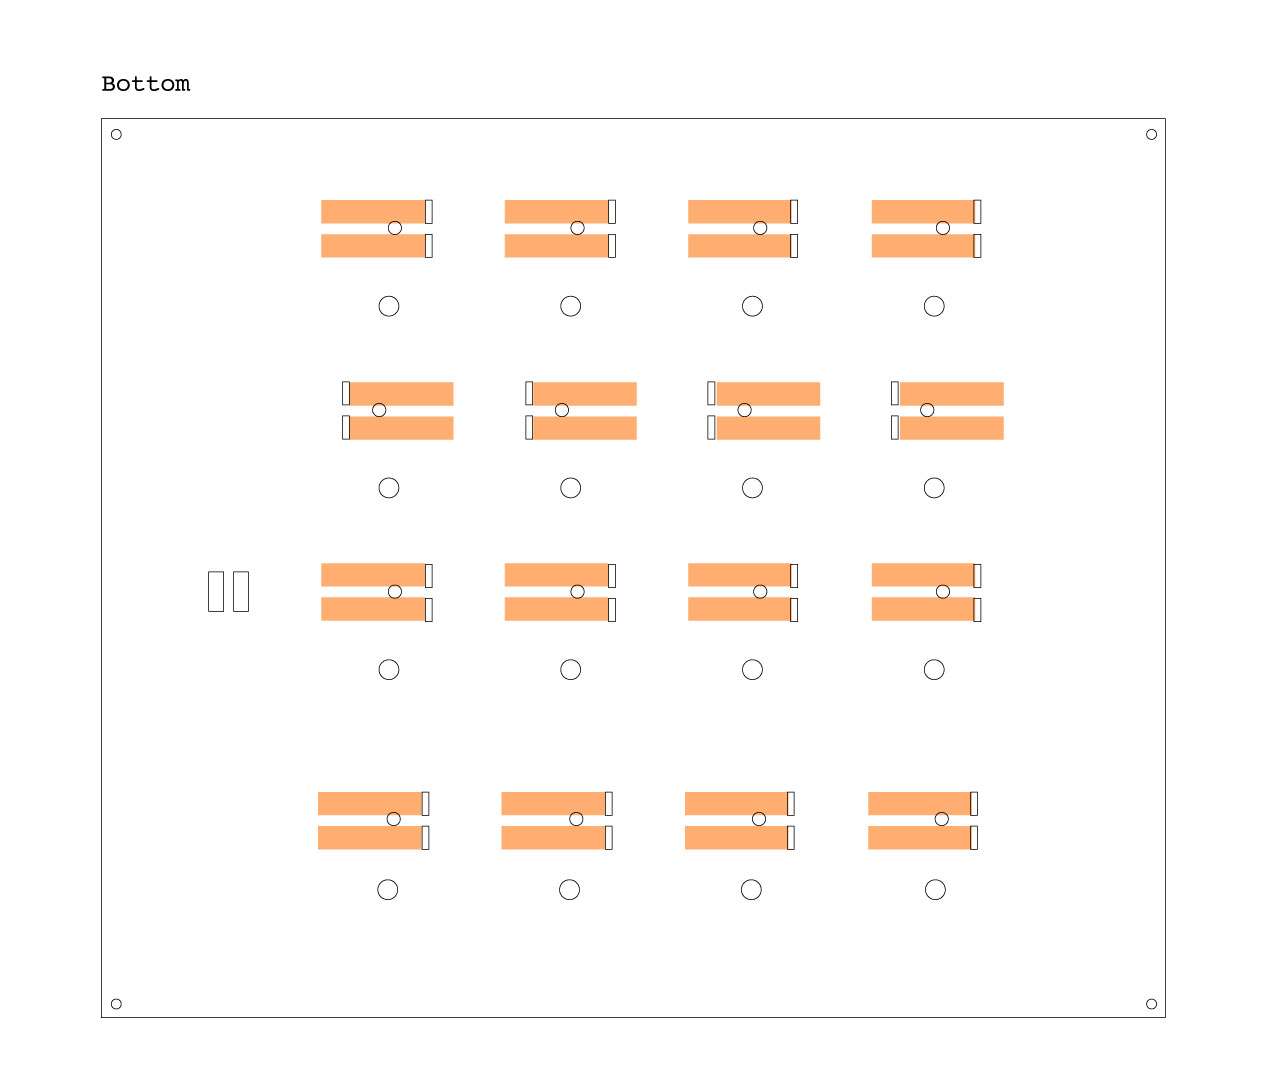
\includegraphics[scale=0.10]{./imagens/board-1.jpg}
 \caption[ ]{Vista da face de baixo dos contatos das peças de instruções}
 %\label{fig:obstaculos}
 \end{figure}

\begin{figure}[h!] % Poderia ser \begin{figure}[posicionamento], onde o posicionamento pode ser h - no local do texto onde foi  o comando, t - no topo da pagina atual ou b - no final da pagina de trabalho.
 \centering
 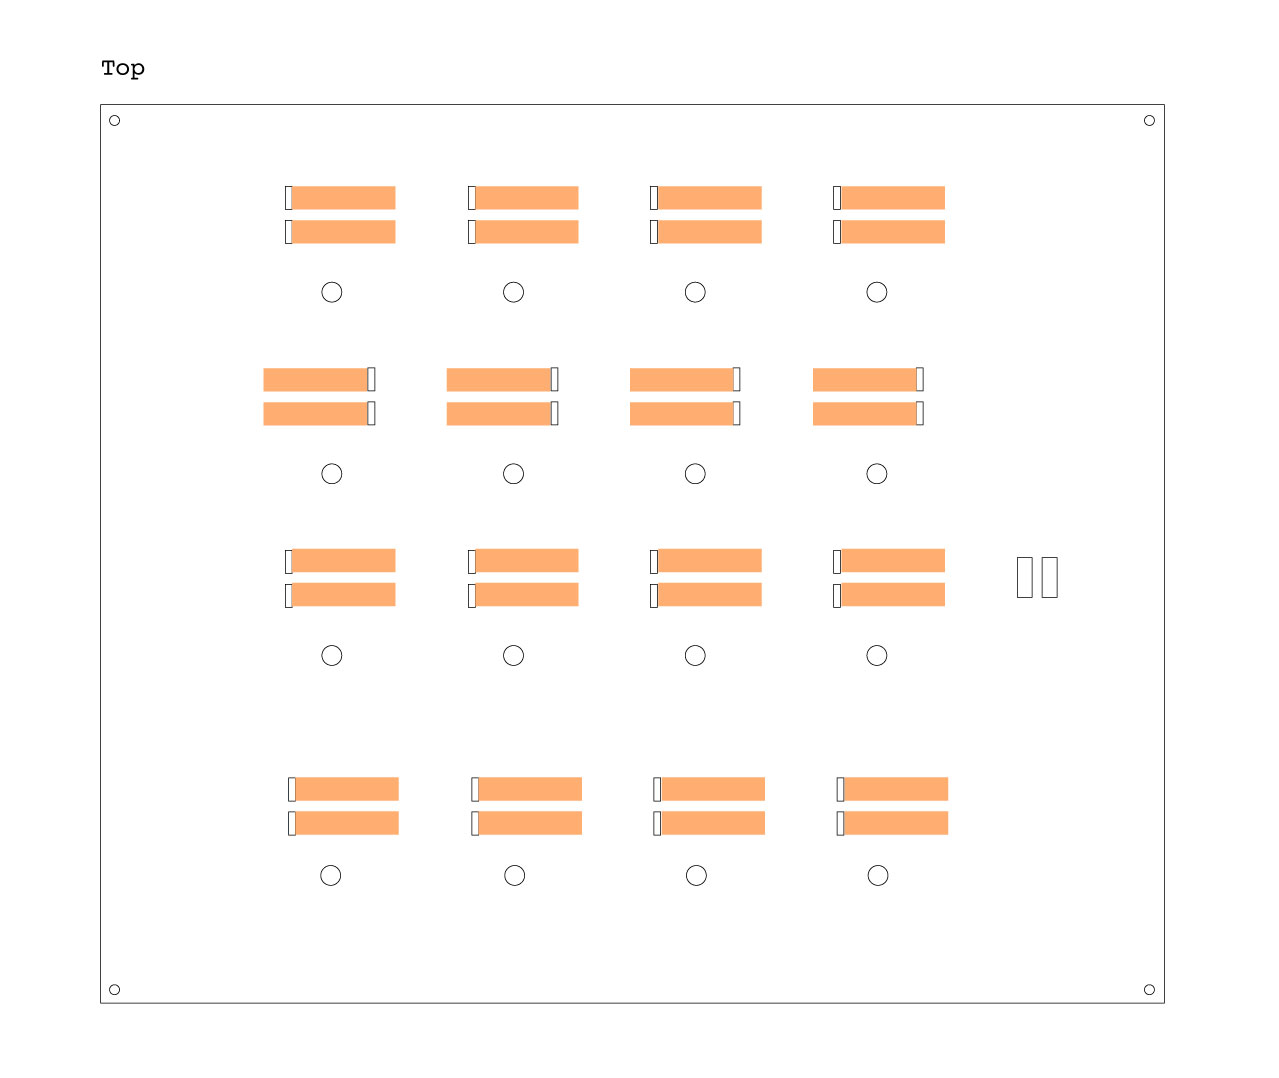
\includegraphics[scale=0.10]{./imagens/board-2.jpg}
 \caption[ ]{Vista da face de cima dos contatos das peças de instruções}
 %\label{fig:obstaculos}
 \end{figure}

Uma vez terminado esse trabalho você pode colar as partes já anteriormente coladas, nessa ordem:1+2 com 3+4.

\begin{figure}[h!] % Poderia ser \begin{figure}[posicionamento], onde o posicionamento pode ser h - no local do texto onde foi  o comando, t - no topo da pagina atual ou b - no final da pagina de trabalho.
 \centering
 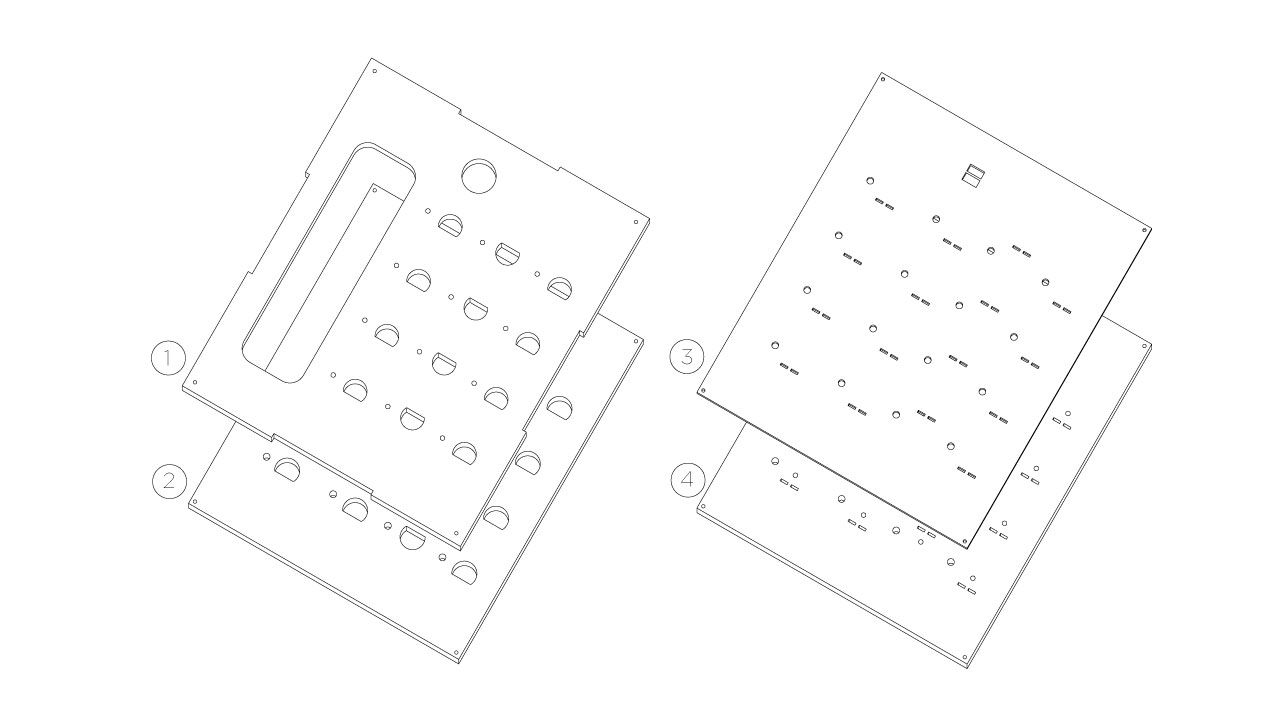
\includegraphics[scale=0.15]{./imagens/board-esploso.jpg}
 \caption[ ]{Peças da mesa de interface}
 %\label{fig:obstaculos}
 \end{figure}
 
 Assim que a cola secar, chegou a hora de colocar os imãs. Vire a camada superior da Mesa para baixo e preencha os pequenos orifícios com os imãs, tendo certeza de que eles estão sempre na mesma polaridade/direção, não importa se norte ou sul. Sele os buraquinhos com uma gota de cola quente.
 
 Agora, a eletrônica! Comece fazendo as trilhas para a alimentação (5V, vermelho) e para o aterramento (GND, preto) em toda a extensão da fila de orifícios, como mostrado na figura \ref{fig:alimentação}. Fizemos o nosso primeiro protótipo sem a fita de cobre, mas usando fios (que você também pode usar), mas nesse protótipo nós preferimos usar a fita, mesmo para as trilhas. Ela deixa o trabalho de montar as conexões muito mais fácil depois.
 
 \begin{figure}[H] % Poderia ser \begin{figure}[posicionamento], onde o posicionamento pode ser h - no local do texto onde foi  o comando, t - no topo da pagina atual ou b - no final da pagina de trabalho.
  \centering
  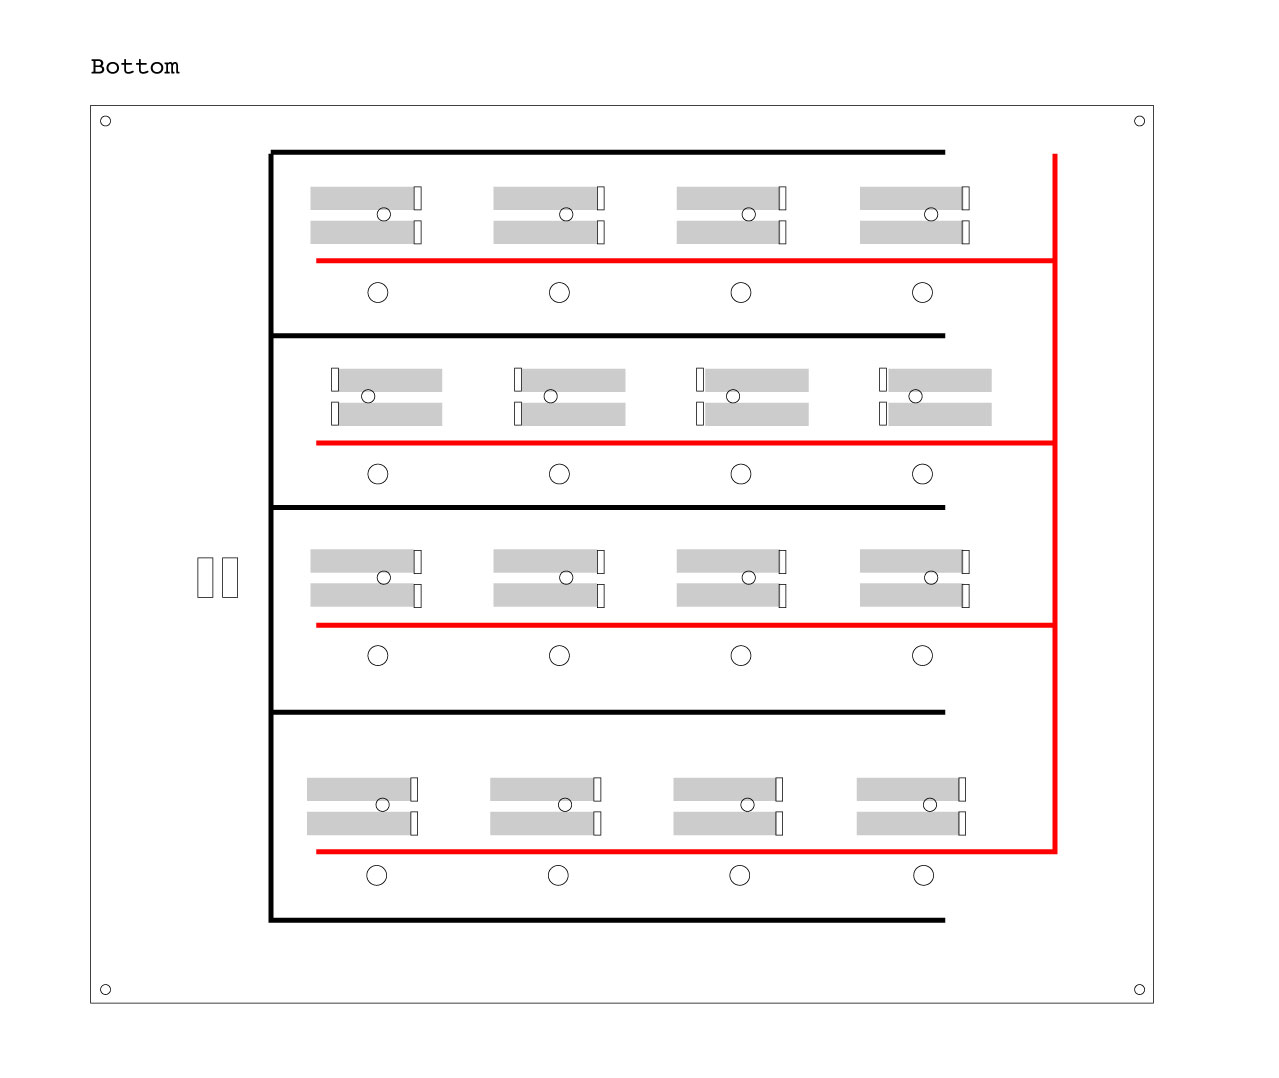
\includegraphics[scale=0.15]{./imagens/board-3.jpg}
  \caption[ ]{Distribuição dos barramentos de alimentação}
  \label{fig:alimentação}
  \end{figure}
  
  O próximo passo é conectar um dos dois conectores de cada orifício à trilha GND. Se você usou a fita de cobre, pode agora usar um pequeno pedaço extra, suficiente apenas para tocar as duas extremidades,\ref{fig:conexão alimentação} .
 
 \begin{figure}[H] % Poderia ser \begin{figure}[posicionamento], onde o posicionamento pode ser h - no local do texto onde foi  o comando, t - no topo da pagina atual ou b - no final da pagina de trabalho.
   \centering
   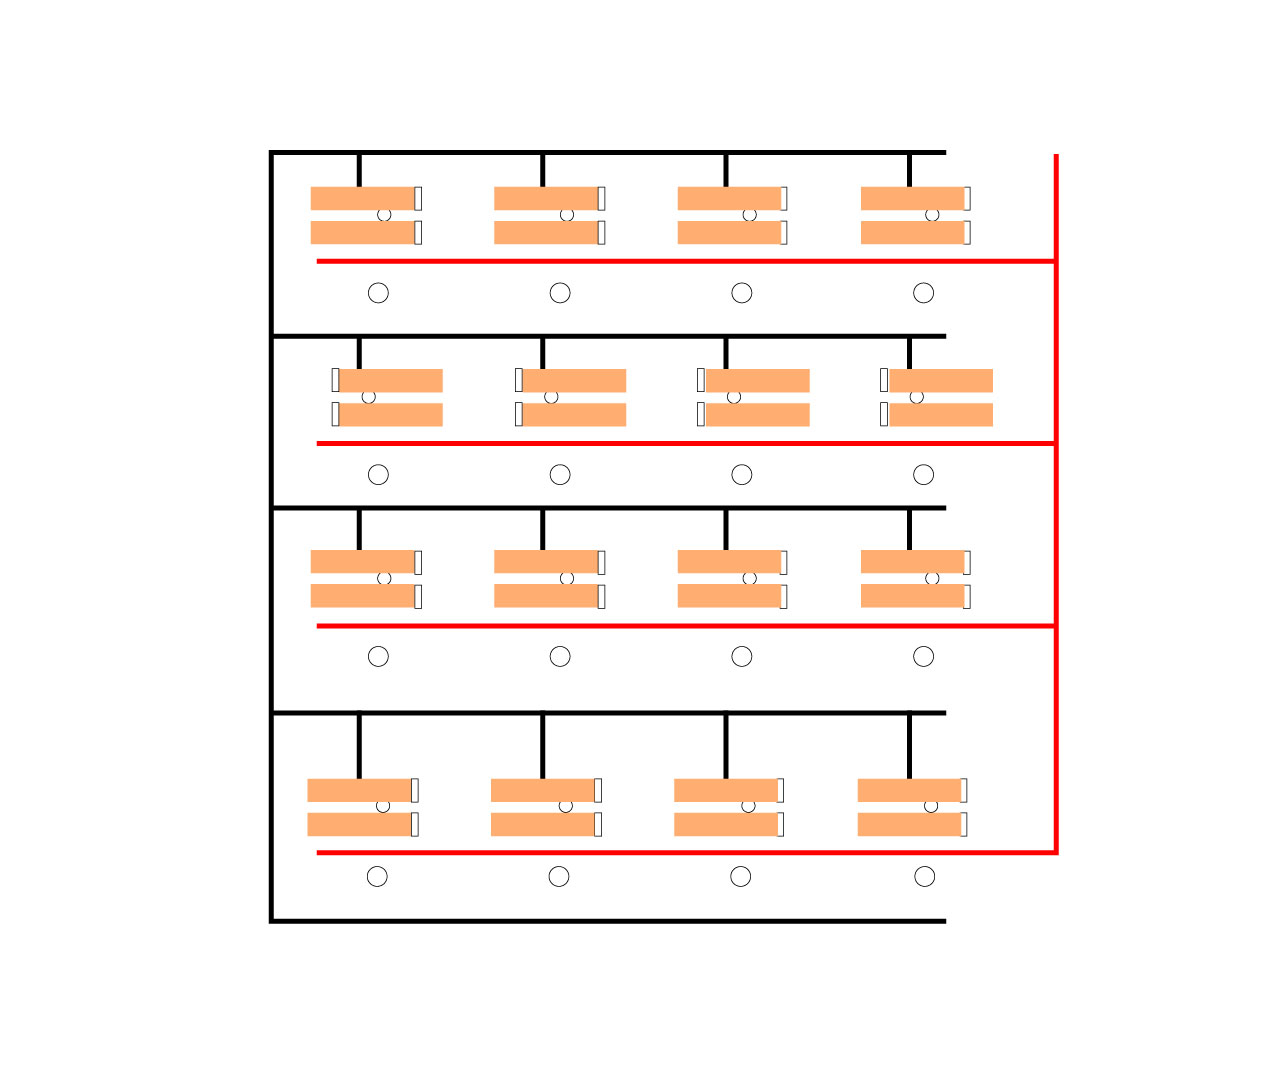
\includegraphics[scale=0.15]{./imagens/board-5.jpg}
   \caption[ ]{Conexão entre os barramentos de alimentação e os contatos }
   \label{fig:conexão alimentação}
   \end{figure}
   
Agora temos que juntar os outros conectores restantes com a trilha de alimentação (5V), mas dessa vez com um resistor de 10K$\Omega$  entre eles. Uma característica bacana da fita de cobre é que a solda gruda muito bem em sua superfície. Essa é a técnica usada,mostrada na Figura \ref{fig:conexão resistor 10k}):   
 
  \begin{figure}[H] % Poderia ser \begin{figure}[posicionamento], onde o posicionamento pode ser h - no local do texto onde foi  o comando, t - no topo da pagina atual ou b - no final da pagina de trabalho.
    \centering
    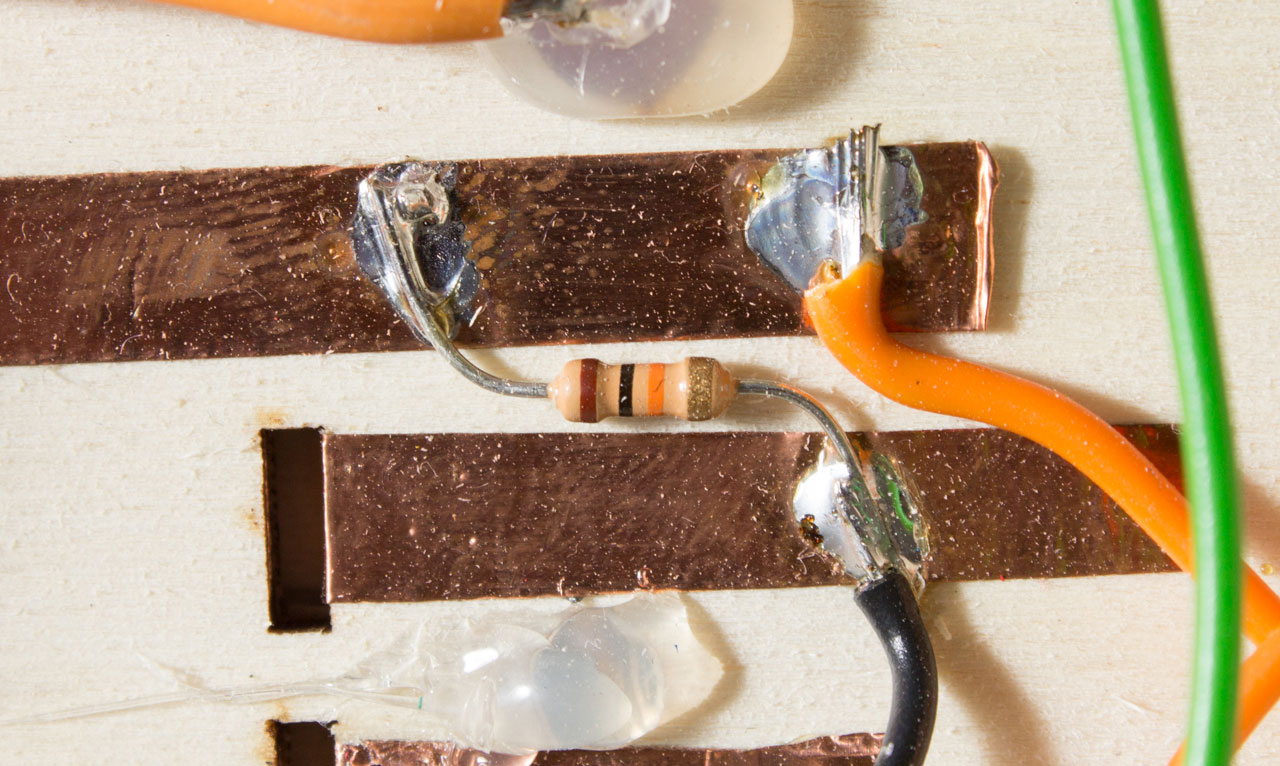
\includegraphics[scale=0.10]{./imagens/diy-docs-1.jpg}
    \caption[ ]{Soldagem do resistor entre os terminais }
    \label{fig:conexão resistor 10k}
   \end{figure}
   
No final desse processo, você deve ter algo assim, ver Figura \ref {fig:esquema com resistores} :

\begin{figure}[h!] % Poderia ser \begin{figure}[posicionamento], onde o posicionamento pode ser h - no local do texto onde foi  o comando, t - no topo da pagina atual ou b - no final da pagina de trabalho.
   \centering
   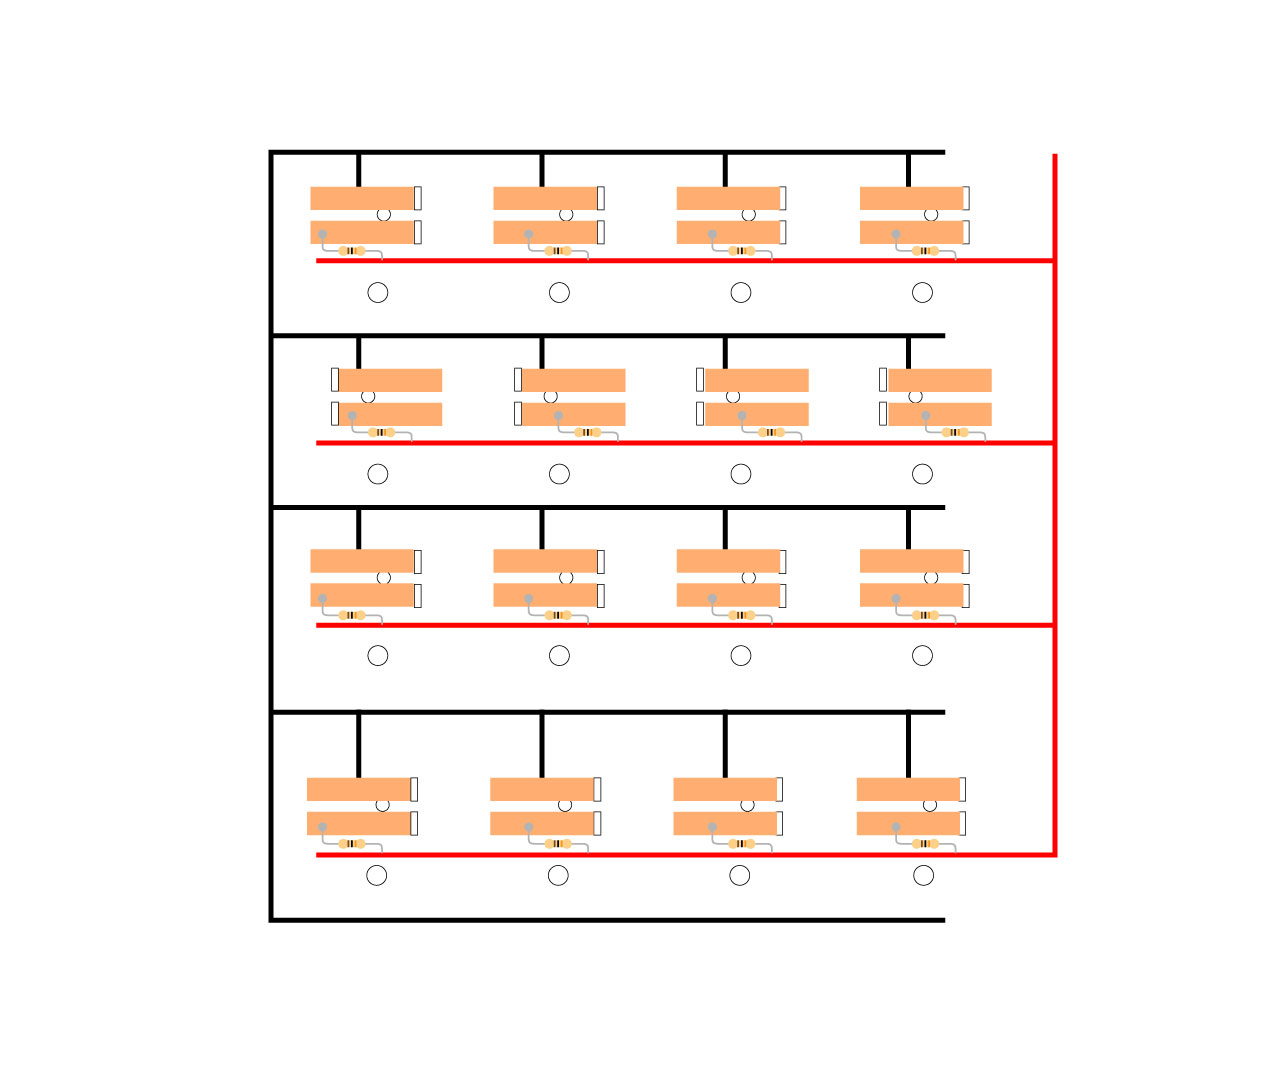
\includegraphics[scale=0.15]{./imagens/board-6.jpg}
   \caption[ ]{Esquema com resistores soldados entre os terminais e alimentação }
   \label{fig:esquema com resistores}
\end{figure}
   
Agora é a hora de colocarmos os LEDs. Espete um LED vermelho em cada um dos 16 orifícios, então use uma gota de cola quente para fixá-los na madeira. Uma vez que a cola esfriou, é a hora de conectá-los. Lembre-se que os LEDs possuem polaridade: a perna mais comprida é o ânodo e a mais curta o cátodo. 

\begin{figure}[h!] % Poderia ser \begin{figure}[posicionamento], onde o posicionamento pode ser h - no local do texto onde foi  o comando, t - no topo da pagina atual ou b - no final da pagina de trabalho.
  \centering
  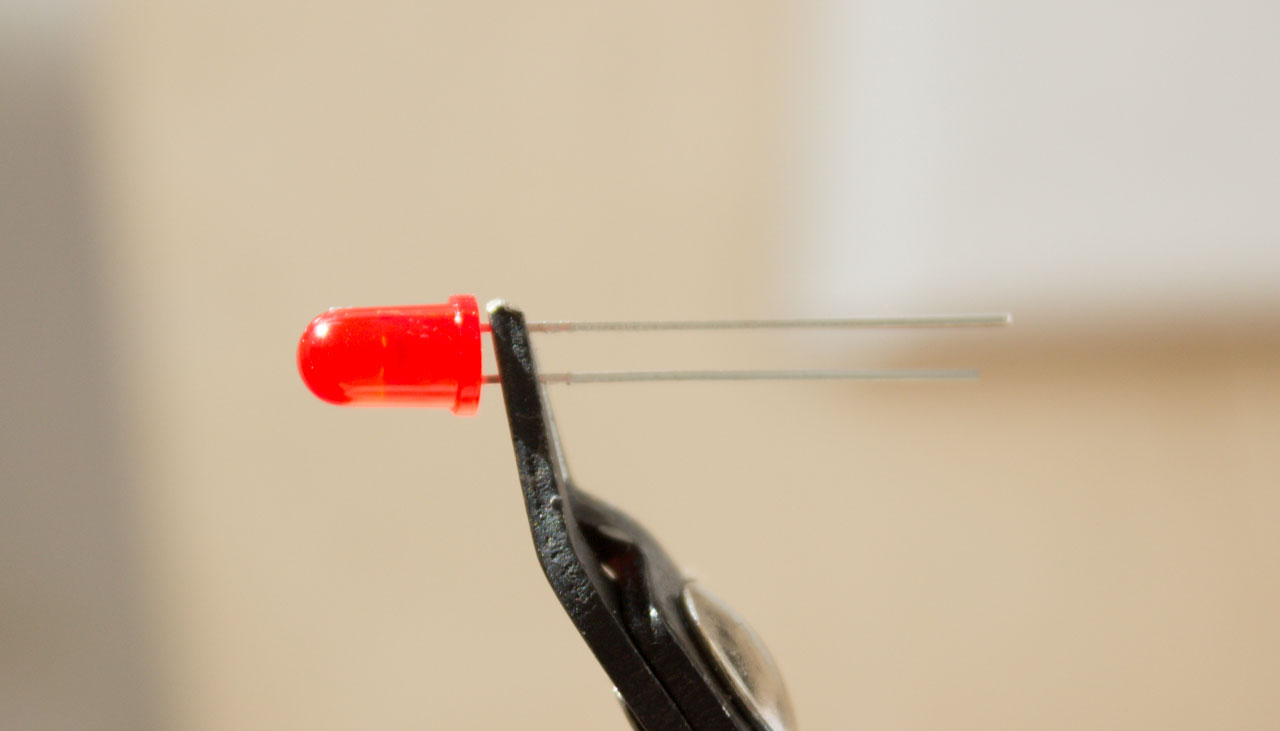
\includegraphics[scale=0.10]{./imagens/diy-docs-6.jpg}
  \caption[ ]{Diferenciação entre ânodo e cátodo }
  \label{fig:termnais led}
\end{figure}

Conecte cada cátodo com a trilha do aterramento (GND), usando um resistor de 220$\Omega$.

\begin{figure}[H] % Poderia ser \begin{figure}[posicionamento], onde o posicionamento pode ser h - no local do texto onde foi  o comando, t - no topo da pagina atual ou b - no final da pagina de trabalho.
  \centering
  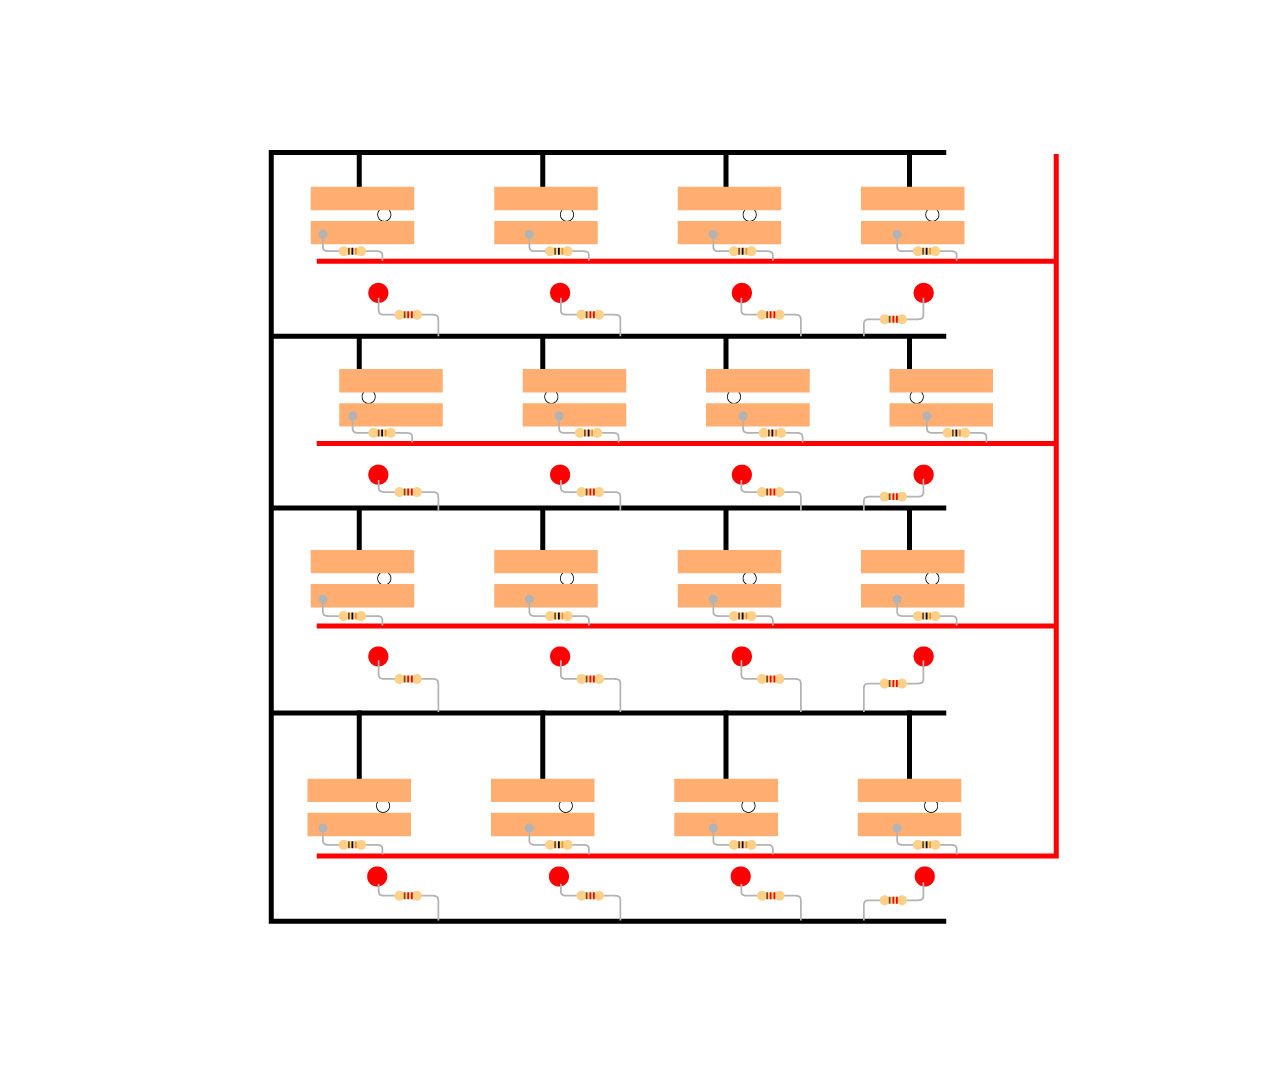
\includegraphics[scale=0.15]{./imagens/board-7.jpg}
  \caption[ ]{Esquema com posicionamento dos LEDs }
  \label{fig:esquemas com leds}
\end{figure}

A perna mais comprida do LED deve ser conectada a um pino de entrada/saída (I/O) digital no Arduino Mega. Esses pinos são numerados de 22 a 53. Os LEDs devem ser conectados numa ordem sequencial, assim será muito mais fácil acessá-los mais tarde durante a programação. No meu protótipo, por exemplo, comecei no pino de número 30 e fui até o 45 (são 16 LEDs).
O ponto de partida não é importante, desde que eles estejam na ordem sequencial correta. Isso significa, por exemplo, que se começarmos do pino 30, o primeiro LED deve estar conectado no pino 30, o segundo no pino 31, o terceiro no pino 32 e assim por diante, até o LED 16 no pino 45.

Os cabos devem ser soldados em uma barra de pinos conectores machos duplos, pois os pinos de entrada e saída no Arduino Mega são dispostos em uma linha dupla. Desta maneira fica mais fácil de remover o Arduino da Mesa de Interface quando for necessário.

\begin{figure}[h!] % Poderia ser \begin{figure}[posicionamento], onde o posicionamento pode ser h - no local do texto onde foi  o comando, t - no topo da pagina atual ou b - no final da pagina de trabalho.
  \centering
  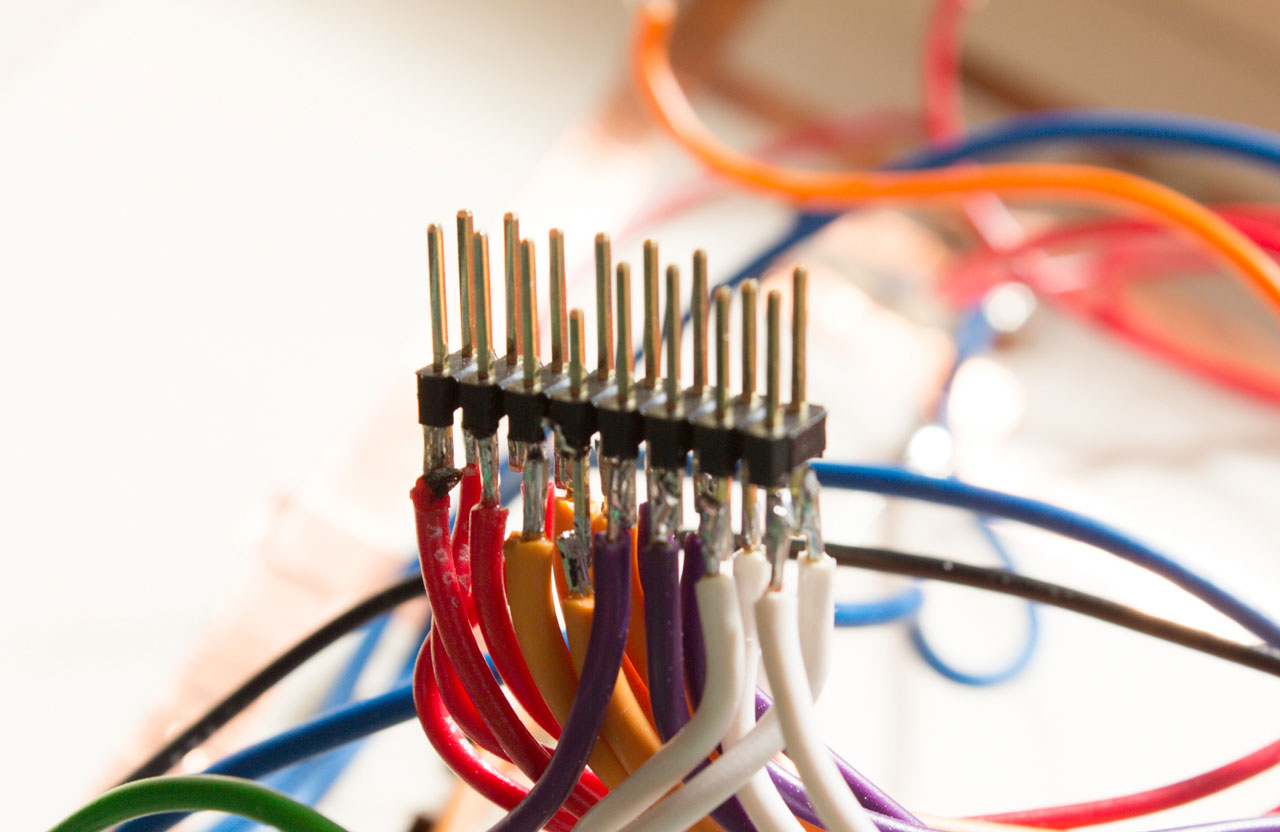
\includegraphics[scale=0.10]{./imagens/diy-docs-4.jpg}
  \caption[ ]{Cabos soldados a conector macho duplo }
  \label{fig:cabos com conector}
\end{figure}

Uma vez que todos os LEDs estejam soldados, nós temos que começar a soldar os conectores da Mesa, àqueles feitos à mão com a fita de cobre. Esses devem ser ligados aos pinos analógicos do Arduino através de um cabo para que seja possível fazer a leitura dos diferentes valores dos resistores. Assim como no caso dos LEDs, esses também dever ser conectados em ordem, começando do A0 para o orifício 1 até o A15 para o orifício 16. O cabo deve ter início do mesmo ponto onde soldamos previamente os resistores de 10K. Veja a imagem:

\begin{figure}[H] % Poderia ser \begin{figure}[posicionamento], onde o posicionamento pode ser h - no local do texto onde foi  o comando, t - no topo da pagina atual ou b - no final da pagina de trabalho.
  \centering
  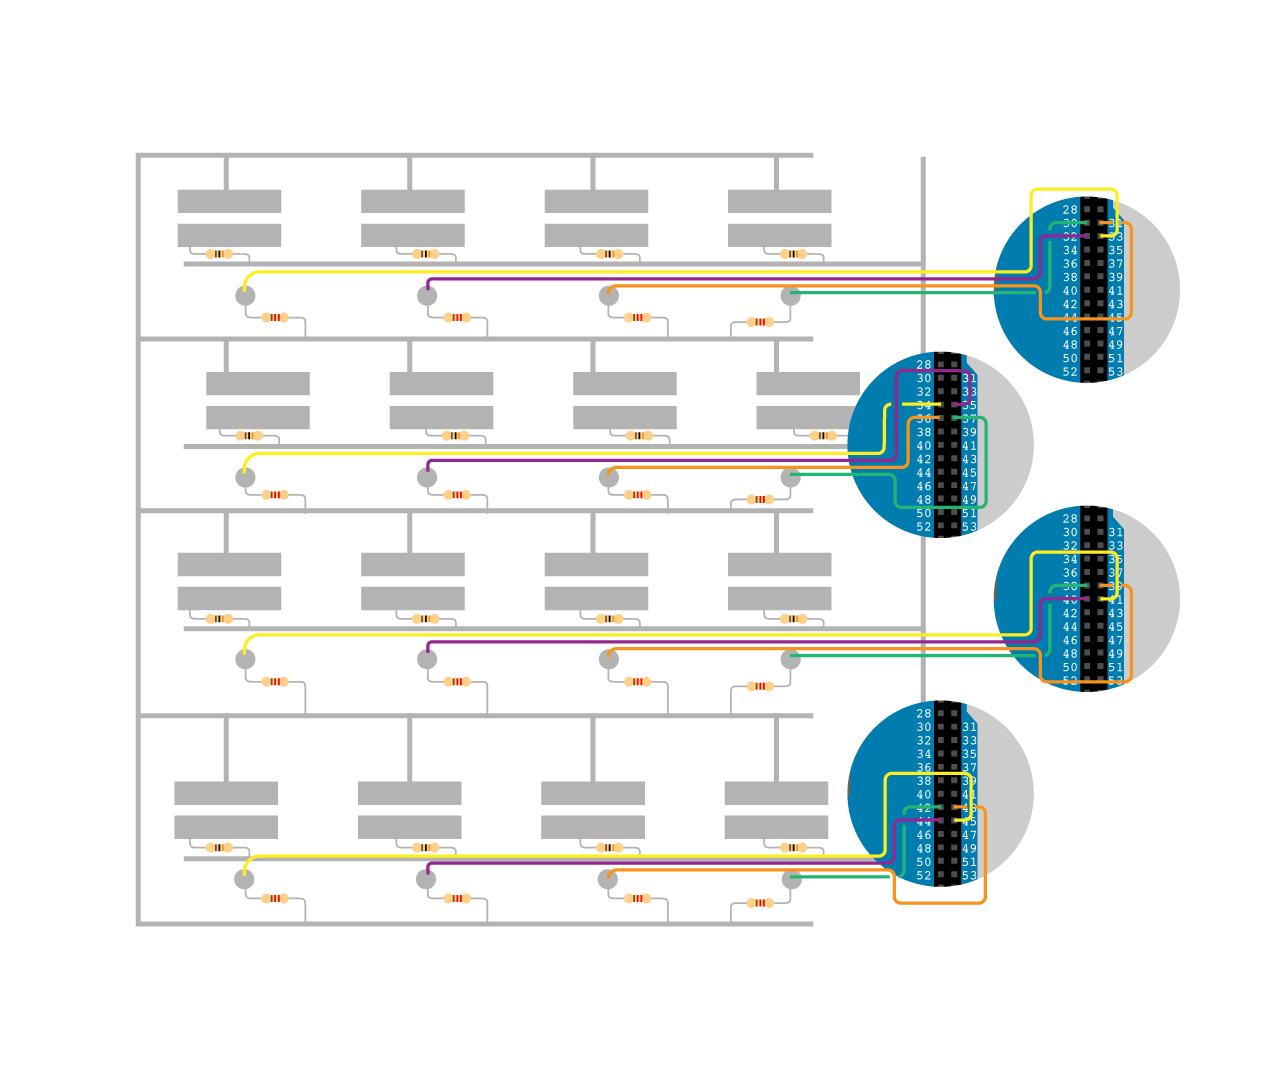
\includegraphics[scale=0.15]{./imagens/board-8.jpg}
  \caption[ ]{Conexão entre contatos dos blocos de instruções e entradas analógicas }
  \label{fig:conexão contato analog-in}
\end{figure}

Aqui eu usei alguns conectores macho simples, já que os pinos de entrada e saída analógicos estão dispostos em apenas uma fileira.

A última coisa a ser conectada é o botão do tipo push-button: solde dois cabos em seus dois conectores, então passe-os pelo seu respectivo orifício na Mesa de Interface, a partir da face superior, puxando-os para baixo até que o botão se encaixe direitinho. Agora vire a Mesa e você deve ter os dois cabos que acabou de soldar saindo pelo orifício. Conecte-os como na figura: um vai direto para a alimentação 5V e o outro para o aterramento (GND) usando um resistor de 10K. Então, conecte-o a um pino de entrada/saída digital no Arduino, a partir de uma extremidade do resistor. Neste exemplo nós usamos o pino de número 50.

\begin{figure}[H] % Poderia ser \begin{figure}[posicionamento], onde o posicionamento pode ser h - no local do texto onde foi  o comando, t - no topo da pagina atual ou b - no final da pagina de trabalho.
  \centering
  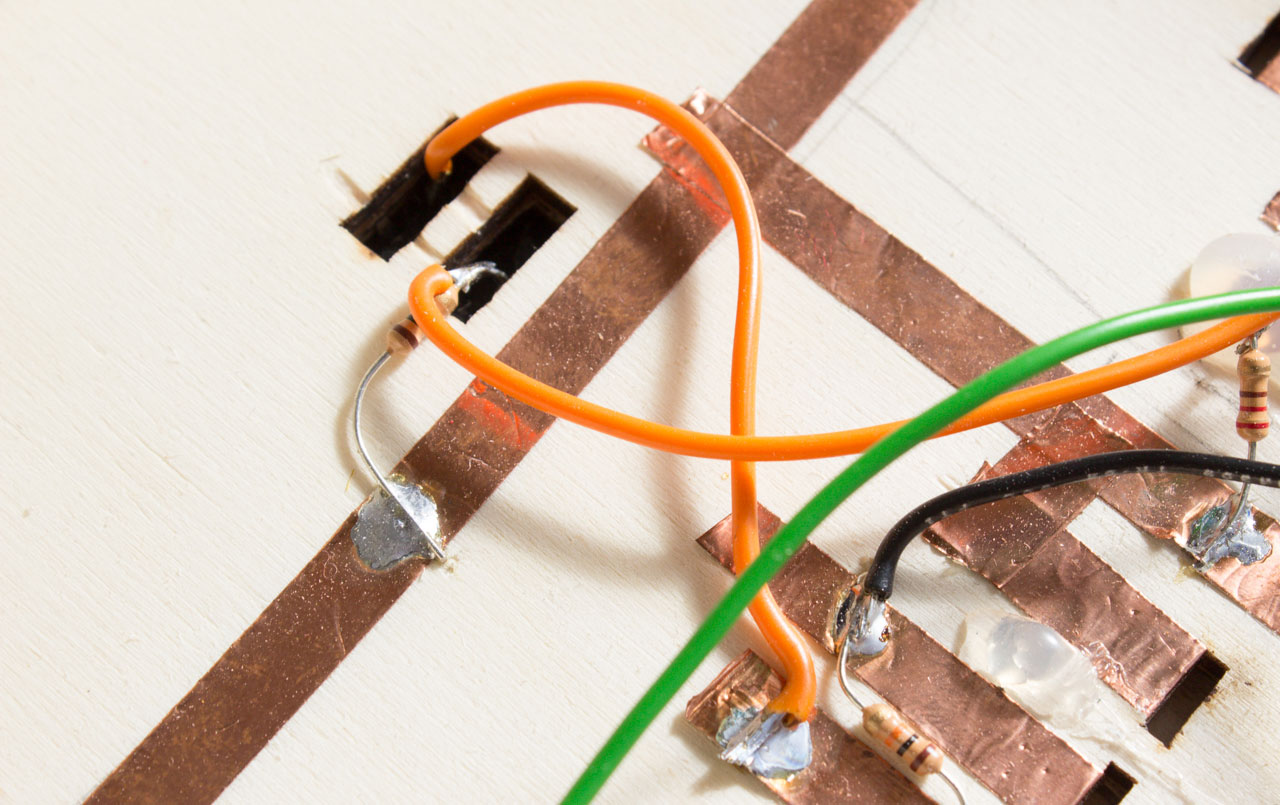
\includegraphics[scale=0.10]{./imagens/diy-docs-5.jpg}
  \caption[ ]{Cabos de conexão do push-botton }
  \label{fig:push-botton}
\end{figure}

A Mesa já está quase pronta, agora só falta conectar o módulo wireless na parte superior do Arduino Mega e plugar os conectores em seu lugar na placa. Recapitulando: pinos 30 a 45 para os LEDs, A0 ao A15 para os conectores e o número 50 para o botão push-button. Use os pinos de A0 a A5 no módulo wireless para os primeiros 5 conectores. Não se esqueça de conectar a trilha do aterramento (GND) ao pino GND e a trilha de alimentação (5V) no pino 5V.

\begin{figure}[h] % Poderia ser \begin{figure}[posicionamento], onde o posicionamento pode ser h - no local do texto onde foi  o comando, t - no topo da pagina atual ou b - no final da pagina de trabalho.
  \centering
  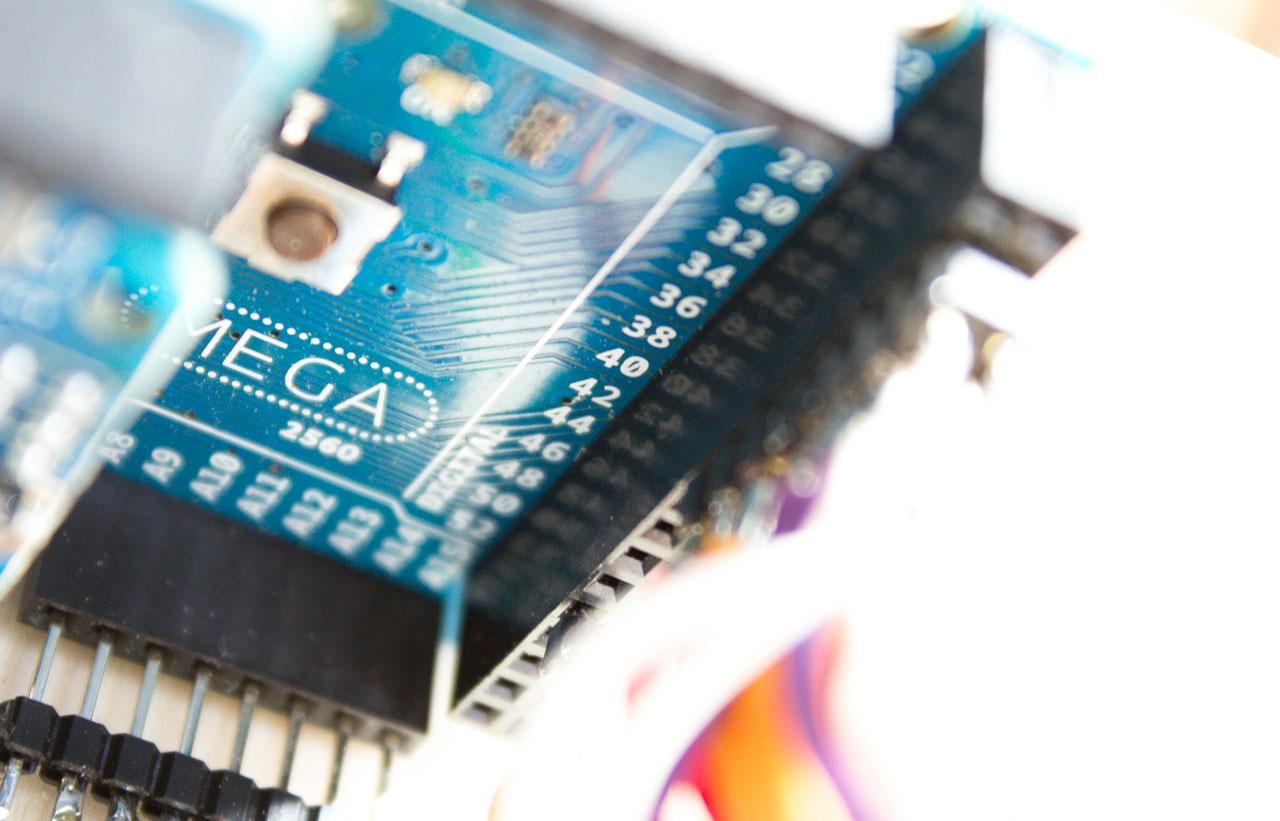
\includegraphics[scale=0.10]{./imagens/diy-docs-3.jpg}
  \caption[ ]{Conexão módulo wireless}
  \label{fig:wifi}
\end{figure}

Agora um ajuste fino: depois de pintar a parte 12 da Mesa, você pode colá-la com a parte 13 no topo da mesma.

O mesmo vale para o botão vermelho: depois de pintar a parte 14, coloque algo macio, como um papel cartão ou EVA no topo da parte 2, ao redor do botão push-button e, antes que a cola seque, cole o botão vermelho. Veja na figura:

\begin{figure}[h] % Poderia ser \begin{figure}[posicionamento], onde o posicionamento pode ser h - no local do texto onde foi  o comando, t - no topo da pagina atual ou b - no final da pagina de trabalho.
  \centering
  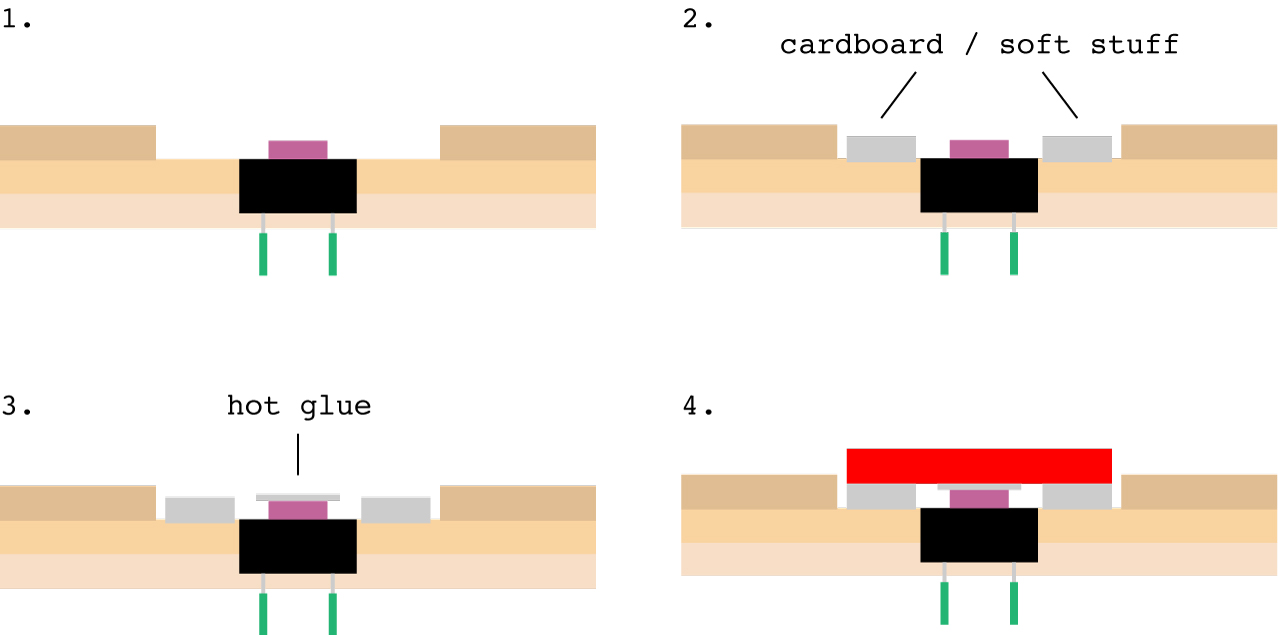
\includegraphics[scale=0.15]{./imagens/button-mechanics.jpg}
  \caption[ ]{Finalização da montagem do push-botton }
  \label{fig:push-botton final}
\end{figure}

\subsection{Bloco de Instruções}

Este é um bloco de instrução, em vista explodida:

\begin{figure}[h] % Poderia ser \begin{figure}[posicionamento], onde o posicionamento pode ser h - no local do texto onde foi  o comando, t - no topo da pagina atual ou b - no final da pagina de trabalho.
  \centering
  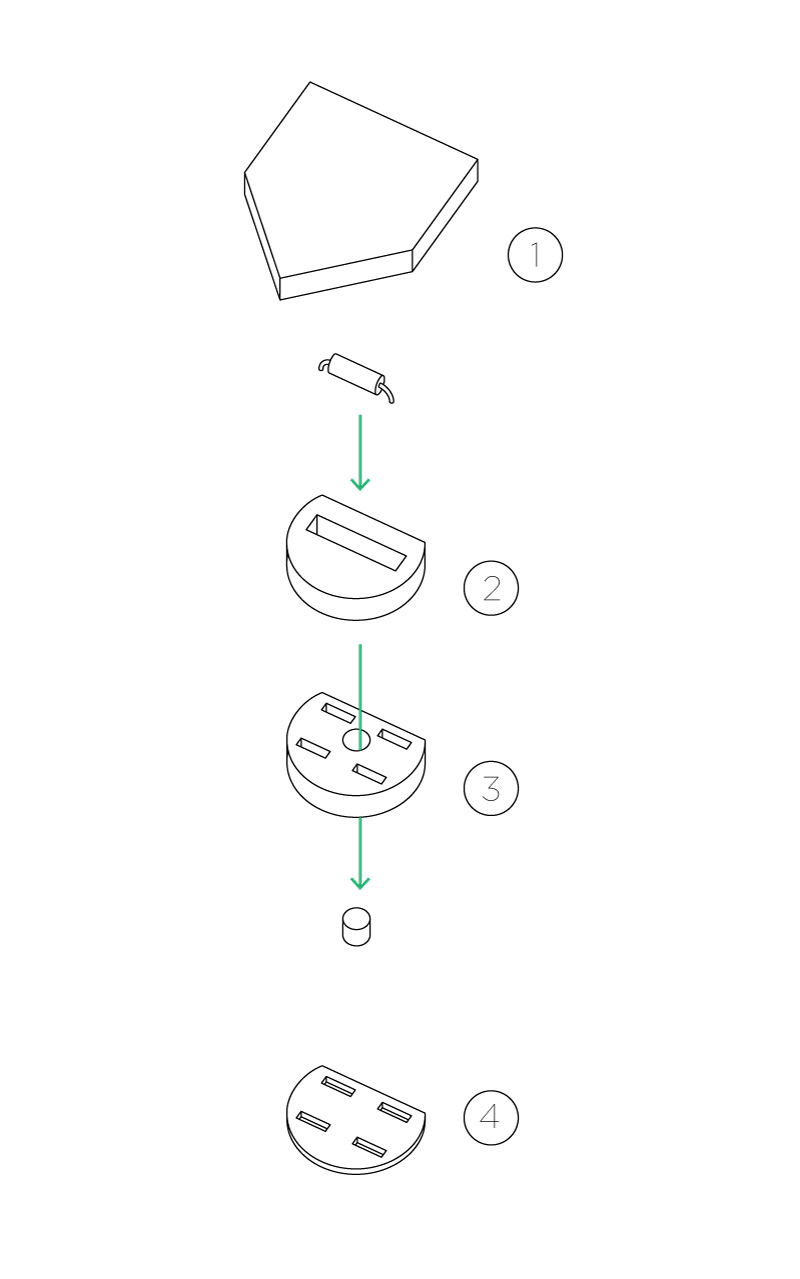
\includegraphics[scale=0.10]{./imagens/instruction-esploso.jpg}
  \caption[ ]{Bloco de instruções: visão explodida }
  \label{fig:bloco explodido}
\end{figure}

Para fazer os Blocos de Instrução, a primeira coisa que você deve providenciar é o corte a laser dos respectivos arquivos; existe um para a madeira de 4mm e um para a de 1mm. São quatro camadas, numeradas de 1 a 4 e os desenhos fornecidos serão usados para fazer 16 blocos, quatro de cada tipo.

Cada bloco possui um resistor diferente. Esses são os valores dos resistores usados no protótipo:

\begin{itemize}
\item FRENTE: 4.7K $\Omega$
\item ESQUERDA: 100K $\Omega$
\item DIREITA: 220 $\Omega$
\item FUNÇÃO: 10K $\Omega$.
\end{itemize}


Para fazer os blocos, primeiro você tem que colar a parte 4 com a parte 3.

Após a cola ter secado, você pode começar a pintar. Veja a figura abaixo para entender o esquema das cores:

\begin{figure}[h] % Poderia ser \begin{figure}[posicionamento], onde o posicionamento pode ser h - no local do texto onde foi  o comando, t - no topo da pagina atual ou b - no final da pagina de trabalho.
  \centering
  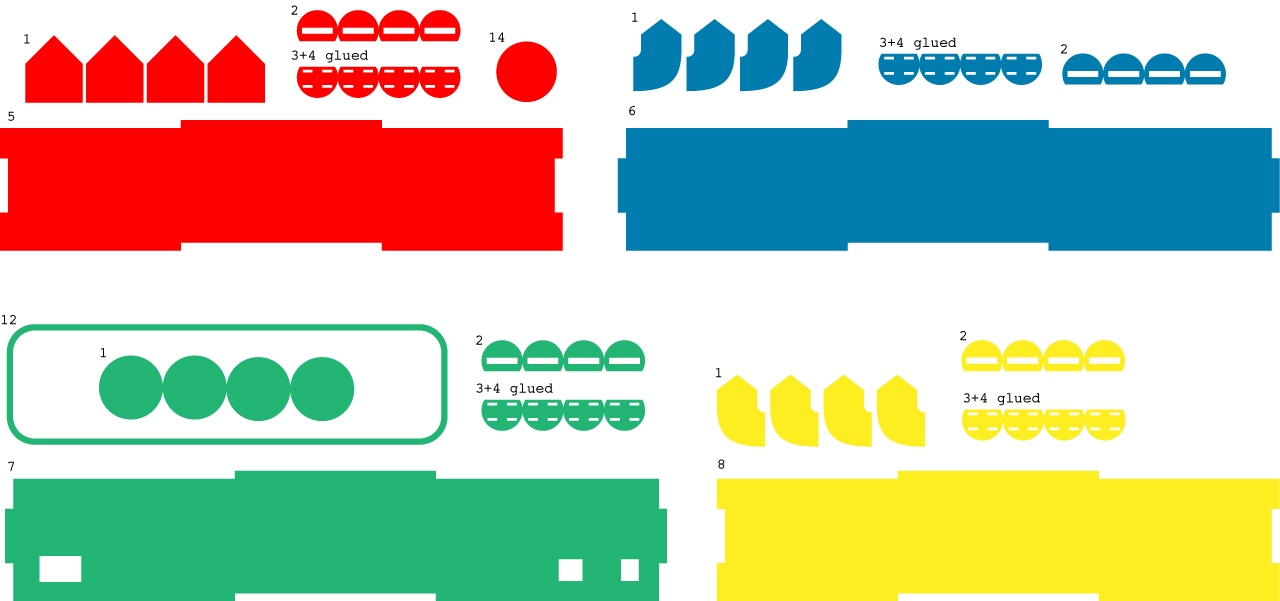
\includegraphics[scale=0.17]{./imagens/colors.jpg}
  \caption[ ]{Esquemas de cores dos blocos de instruções }
  \label{fig:bloco cor}
\end{figure}

Agora você tem que cortar dois pedaços de fita de cobre com 40mm de comprimento. Passe os mesmos pelos orifícios das duas peças que você acabou de colar e forme um anel bem apertado em volta delas.

\begin{figure}[H] % Poderia ser \begin{figure}[posicionamento], onde o posicionamento pode ser h - no local do texto onde foi  o comando, t - no topo da pagina atual ou b - no final da pagina de trabalho.
  \centering
  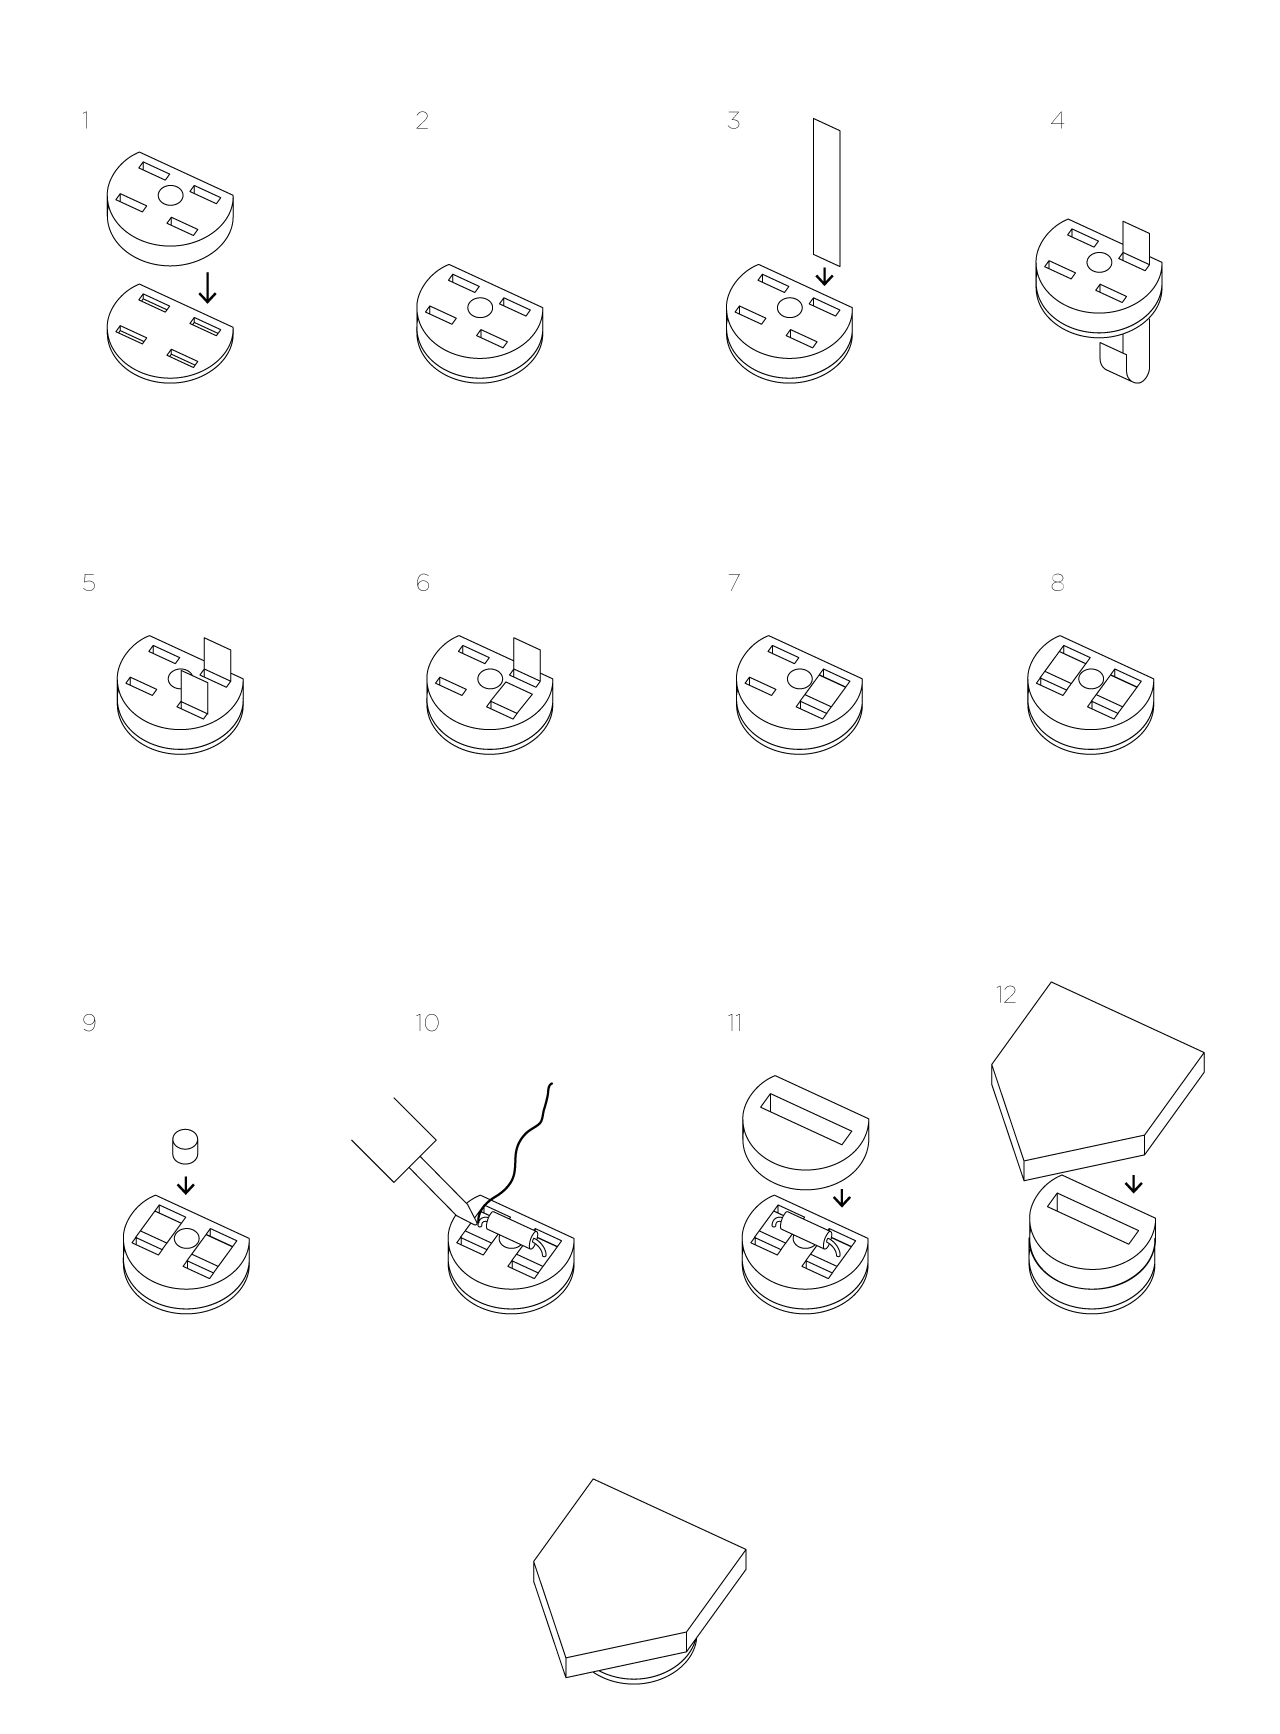
\includegraphics[scale=0.15]{./imagens/instruction-block-guide.jpg}
  \caption[ ]{Montagem dos blocos de instruções }
  \label{fig:bloco montagem}
\end{figure}

Depois disso você deve inserir os imãs dentro dos orifícios. Enquanto faz isso, \textbf{TENHA CERTEZA QUE OS MESMOS ESTÃO CORRETAMENTE ORIENTADOS}, para que os blocos de fato ’grudem’ na Mesa. Se você fizer de maneira contrária os mesmos serão repelidos, o que é até engraçado, mas não é o que queremos, certo?

Fixe o imã com uma gota de cola quente e, antes da cola esfriar, coloque o resistor correspondente no topo, com os terminais ("pernas") sobre a fita de cobre. Depois disso, o resistor precisa ser soldado nessas duas partes. Depois de soldar, corte a parte que sobrou e cole a parte 2 no topo do resistor.

Termine seu bloco colando a última camada, a parte número 1, no topo, e repita todo o processo para cada Bloco de Instrução.

\subsection{CUBETTO}

\textbf{Eletrônica:}

O protótipo do Cubetto pode ser construído usando um Arduino Uno ou Leonardo, com um Módulo Wireless agregado. A razão do uso desse tipo de módulo é que ele tem uma superfície relativamente pequena, mas que é suficiente para colocarmos os drivers dos motores, os conectores para os codificadores ópticos, os motores e a alimentação. 

O Cubetto deve girar 90 graus para a esquerda e para a direita. Uma maneira não muito precisa de fazer isso seria usando uma contagem de tempo, fazendo algo como “gire a direita por um segundo”. É de se esperar que o resultado seja mais ou menos sempre o mesmo. “Mais ou menos” porque isso vai depender de uma porção de fatores distintos, como o piso, a carga da bateria e assim por diante. A maneira que resolvemos esse problema é detectando a quantidade de rotação da roda usando dois sensores ópticos CNY70 combinados com um adesivo. O adesivo redondo é aplicado por dentro da roda, como na Figura \ref {fig:encoder} :

\begin{figure}[h] % Poderia ser \begin{figure}[posicionamento], onde o posicionamento pode ser h - no local do texto onde foi  o comando, t - no topo da pagina atual ou b - no final da pagina de trabalho.
  \centering
  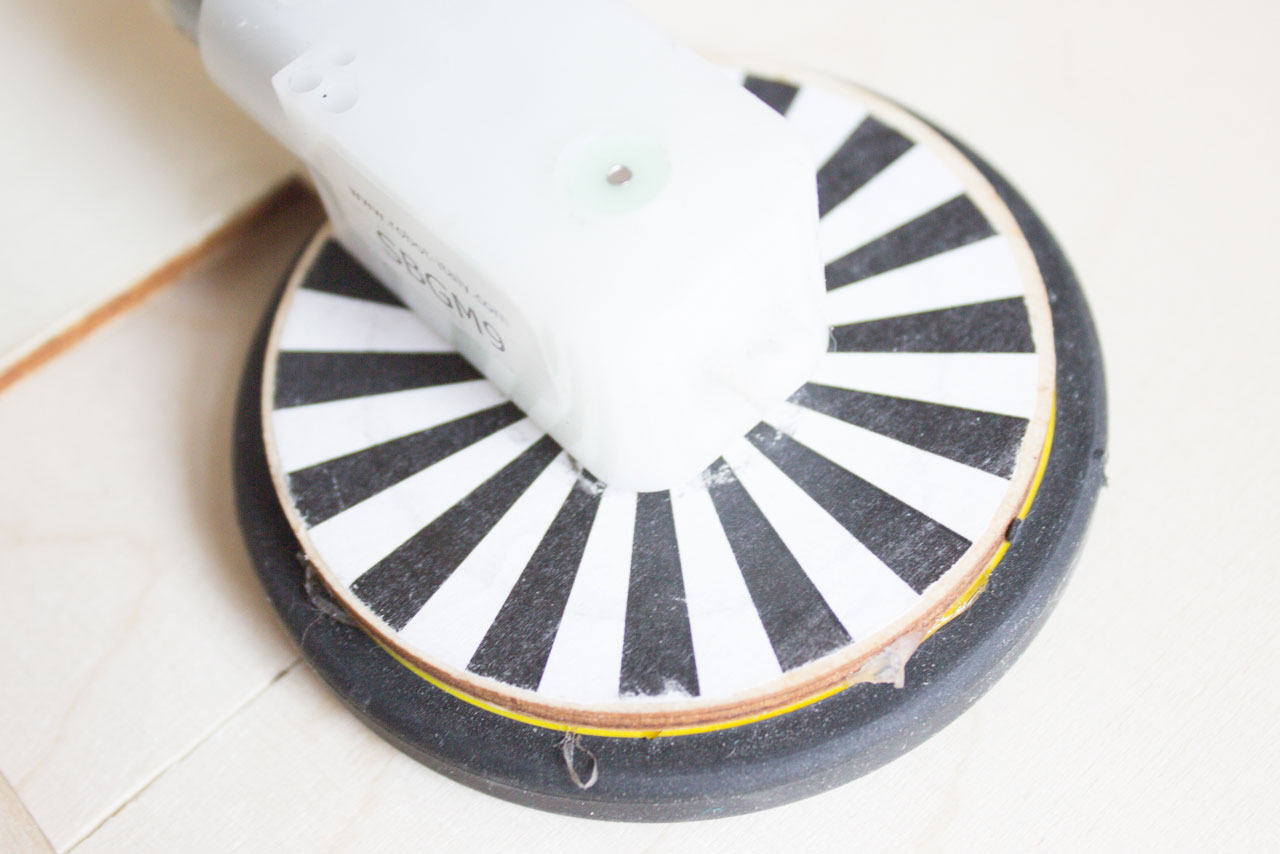
\includegraphics[scale=0.10]{./imagens/diy-docs-14.jpg}
  \caption[ ]{Imagem do adesivo na roda para montar o encoder }
  \label{fig:encoder}
\end{figure}

O adesivo tem um padrão geométrico de listas pretas e brancas, porque o CNY70 é capaz de detectar a variação da emissão de entre elas. Dentro deles, basicamente existe um LED infravermelho - sempre ligado - e um fototransistor que faz a leitura da quantidade de luz infravermelha. Quando o material preto está na frente do componente quase não há luz refletida, já que a cor preta tende a absorvê-la. No caso oposto, quando o material é branco, ele reflete toda a luz, logo o valor lido pelo sensor é muito grande. A diferença entre essas leituras é usada para controlar a quantidade de rotação.

\begin{figure}[h] % Poderia ser \begin{figure}[posicionamento], onde o posicionamento pode ser h - no local do texto onde foi  o comando, t - no topo da pagina atual ou b - no final da pagina de trabalho.
  \centering
  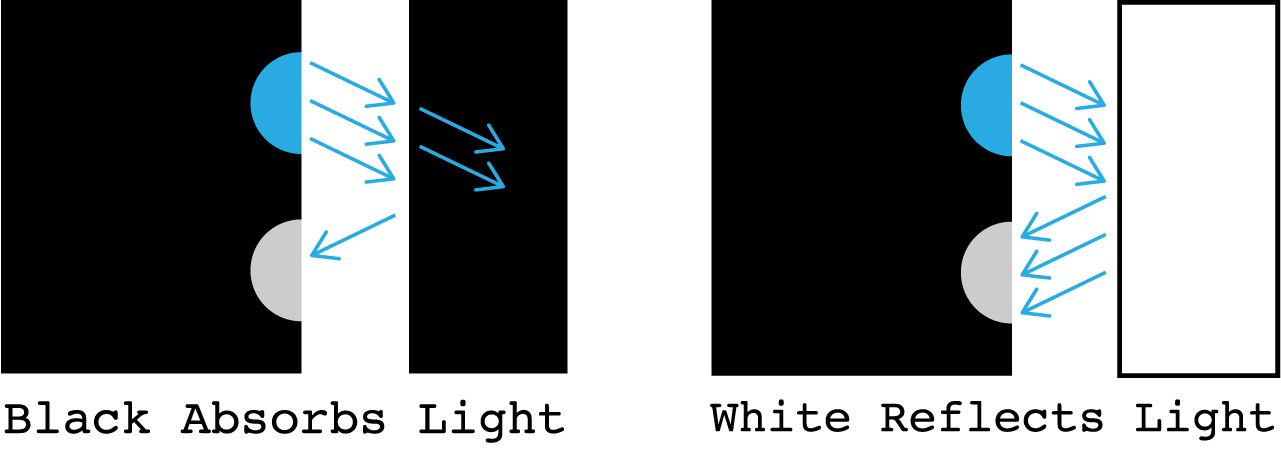
\includegraphics[scale=0.10]{./imagens/cny70-physycs.jpg}
  \caption[ ]{Esquema de funcionamento do CNY70 }
  \label{fig:cny70}
\end{figure}

A área útil disponível no Módulo Wireless é onde os drivers dos motores e outros conectores das demais peças serão soldados. 

\begin{figure}[h] % Poderia ser \begin{figure}[posicionamento], onde o posicionamento pode ser h - no local do texto onde foi  o comando, t - no topo da pagina atual ou b - no final da pagina de trabalho.
  \centering
  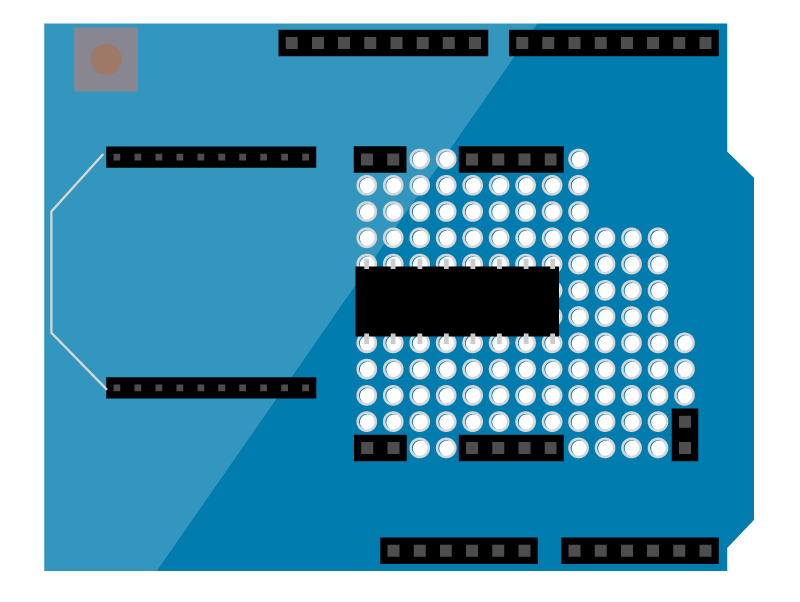
\includegraphics[scale=0.13]{./imagens/wireless-shield-connections.jpg}
  \caption[ ]{Shield de módulo wireless com driver de motor }
  \label{fig:esquema shield}
\end{figure}

O driver de motor SN754410 possui 16 pinos, que devem ser conectados seguindo esse esquema:

\begin{figure}[h] % Poderia ser \begin{figure}[posicionamento], onde o posicionamento pode ser h - no local do texto onde foi  o comando, t - no topo da pagina atual ou b - no final da pagina de trabalho.
  \centering
  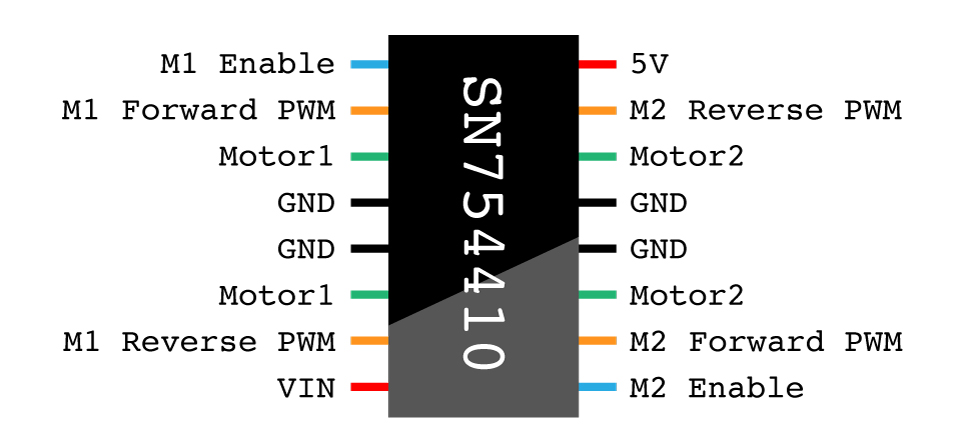
\includegraphics[scale=0.15]{./imagens/motor-driver.jpg}
  \caption[ ]{Conexões do SN754410 }
  \label{fig:conexao ci}
\end{figure}

\textbf{Design:}

Começe cortando a laser o arquivo cubetto.dxf. Todas as partes do Cubetto são feitas com compensado de 4mm. Siga essas instruções para montar a base:

\begin{figure}[h] % Poderia ser \begin{figure}[posicionamento], onde o posicionamento pode ser h - no local do texto onde foi  o comando, t - no topo da pagina atual ou b - no final da pagina de trabalho.
  \centering
  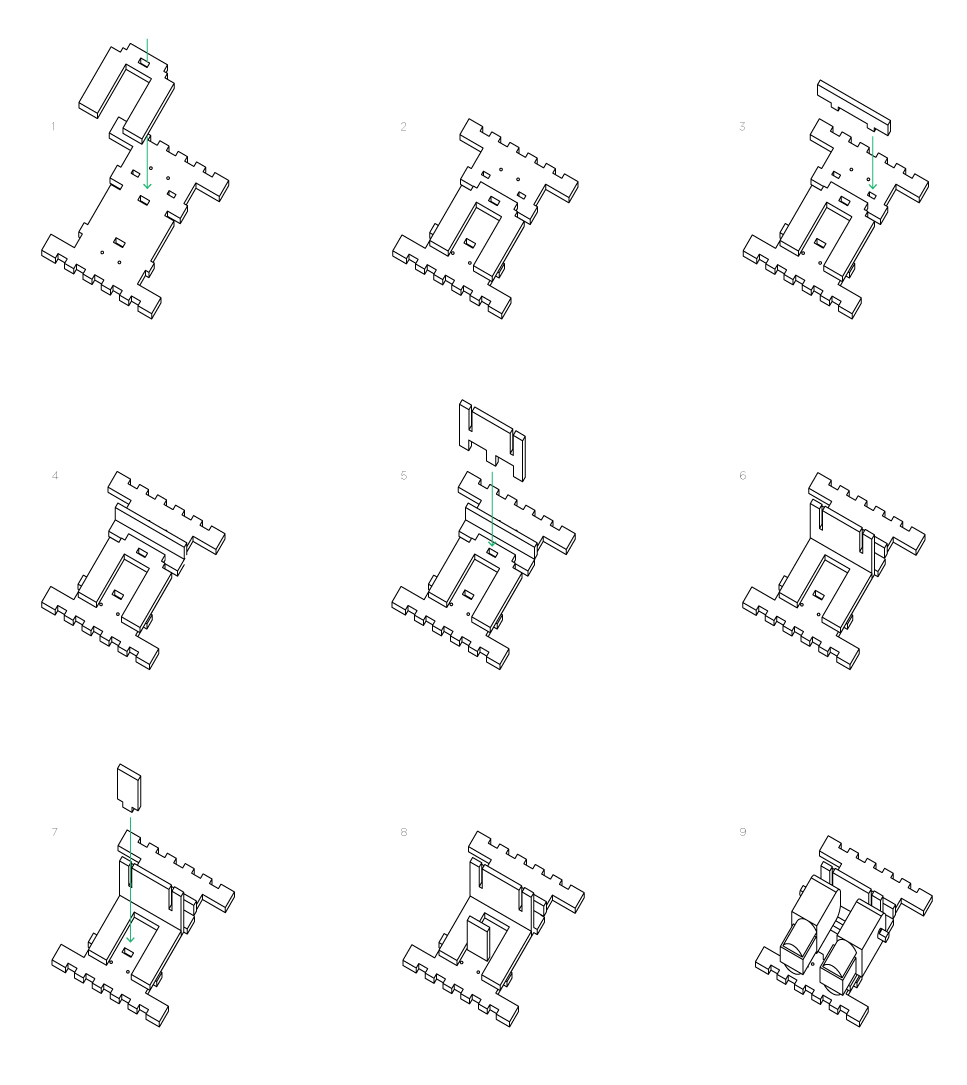
\includegraphics[scale=0.15]{./imagens/cubetto-guide.jpg}
  \caption[ ]{Esquema de montagem da estrutura do Cubetto }
  \label{fig:montagem cubetto}
\end{figure}

Ainda não monte os motores, você precisa primeiro montar os rodízios de metal!

\begin{figure}[h] % Poderia ser \begin{figure}[posicionamento], onde o posicionamento pode ser h - no local do texto onde foi  o comando, t - no topo da pagina atual ou b - no final da pagina de trabalho.
  \centering
  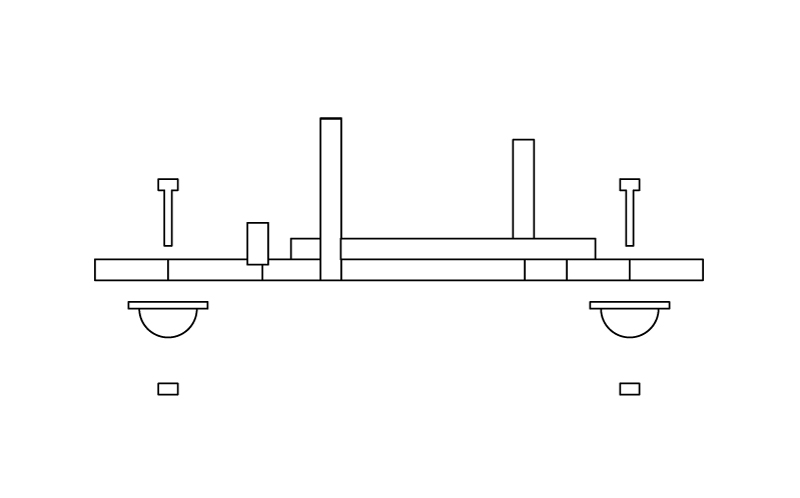
\includegraphics[scale=0.12]{./imagens/ball-caster.jpg}
  \caption[ ]{Montagem do rodízio de metal }
  \label{fig:montagem rodizio}
\end{figure}

\begin{figure}[H] % Poderia ser \begin{figure}[posicionamento], onde o posicionamento pode ser h - no local do texto onde foi  o comando, t - no topo da pagina atual ou b - no final da pagina de trabalho.
  \centering
  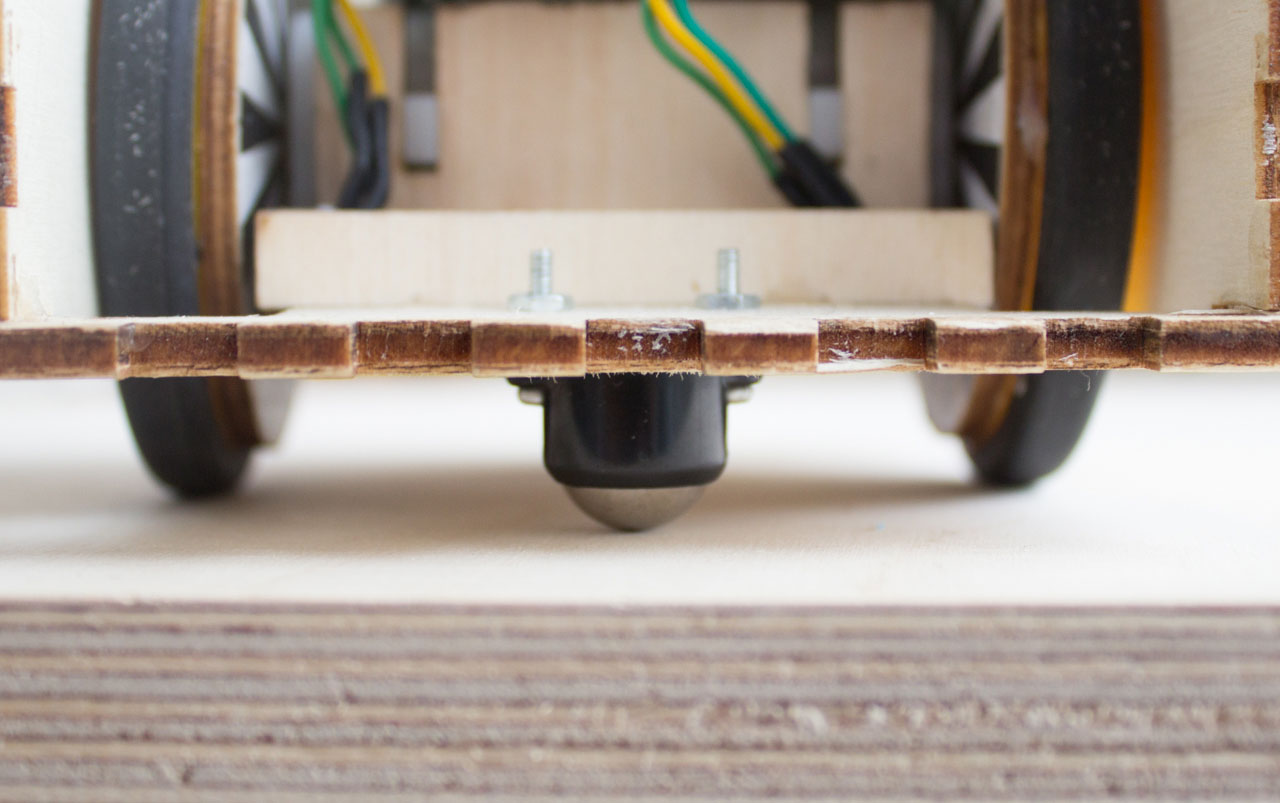
\includegraphics[scale=0.10]{./imagens/diy-docs-9.jpg}
  \caption[ ]{Imagem do rodízio montado }
  \label{fig:foto rodizio}
\end{figure}

Agora vamos cuidar do CNY70. Solde os dois conectores opostos, que devem ser ligados à alimentação 5V, juntamente através de um mesmo fio; então solde mais três fios nos conectores restantes do CNY70. No final desses fios, solde um bloco de três conectores fêmeas. Eles serão conectados mais tarde aos seus pares no Módulo Wireless.

Os dois CNY70 devem ser colocados na beirada da camada inferior, com o LED e o fototransistor alinhados horizontalmente. Para fixá-los você pode usar um pouco de cola quente, ou de qualquer outro tipo de cola.

Veja a Figura \ref{fig:cny70 no cubetto} para entender bem a posição.


\begin{figure}[h] % Poderia ser \begin{figure}[posicionamento], onde o posicionamento pode ser h - no local do texto onde foi  o comando, t - no topo da pagina atual ou b - no final da pagina de trabalho.
  \centering
  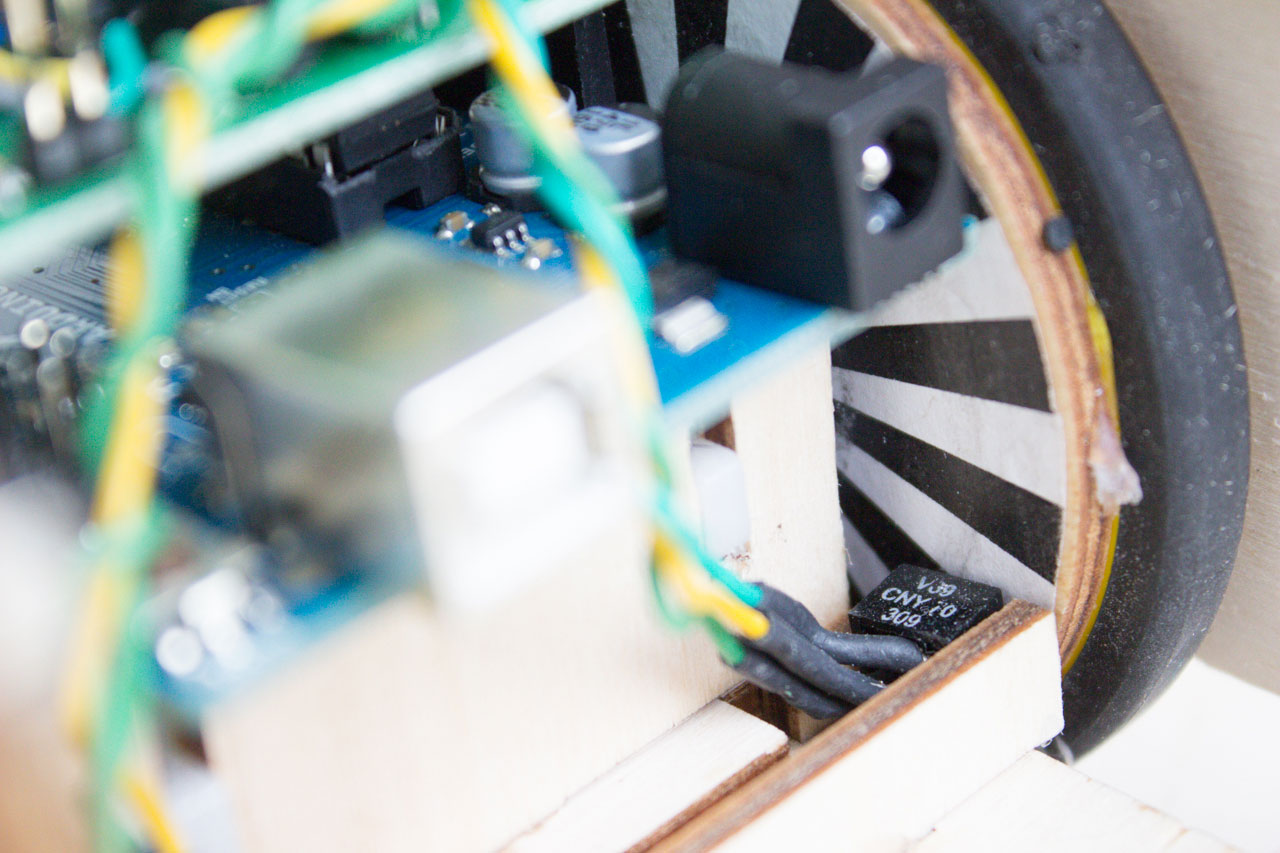
\includegraphics[scale=0.10]{./imagens/diy-docs-11.jpg}
  \caption[ ]{Foto do CNY70 montado no Cubetto }
  \label{fig:cny70 no cubetto}
\end{figure}

Assim como nos CNY70, solde dois cabos às pequenas abas que saem de cada motor. Você pode torcer os dois cabos para fazê-los ficar um pouco mais resistentes e então, no final, solde um bloco de dois conectores fêmeas, como você pode ver na figura.

Agora imprima o desenho com as listas pretas e brancas e cole-o em um pedaço de cartolina (ou numa madeira fina também cortada a laser, fica a seu critério). Corte o perímetro e faça um furo bem no meio, pois ele será inserido entre o motor e a roda. As listas pretas e brancas devem estar viradas para o lado de dentro do Cubetto e a distância entre elas e o sensor CNY70 deve ser algo em torno de 1 a 3mm, para que o CNY70 funcione corretamente.

\begin{figure}[H] % Poderia ser \begin{figure}[posicionamento], onde o posicionamento pode ser h - no local do texto onde foi  o comando, t - no topo da pagina atual ou b - no final da pagina de trabalho.
  \centering
  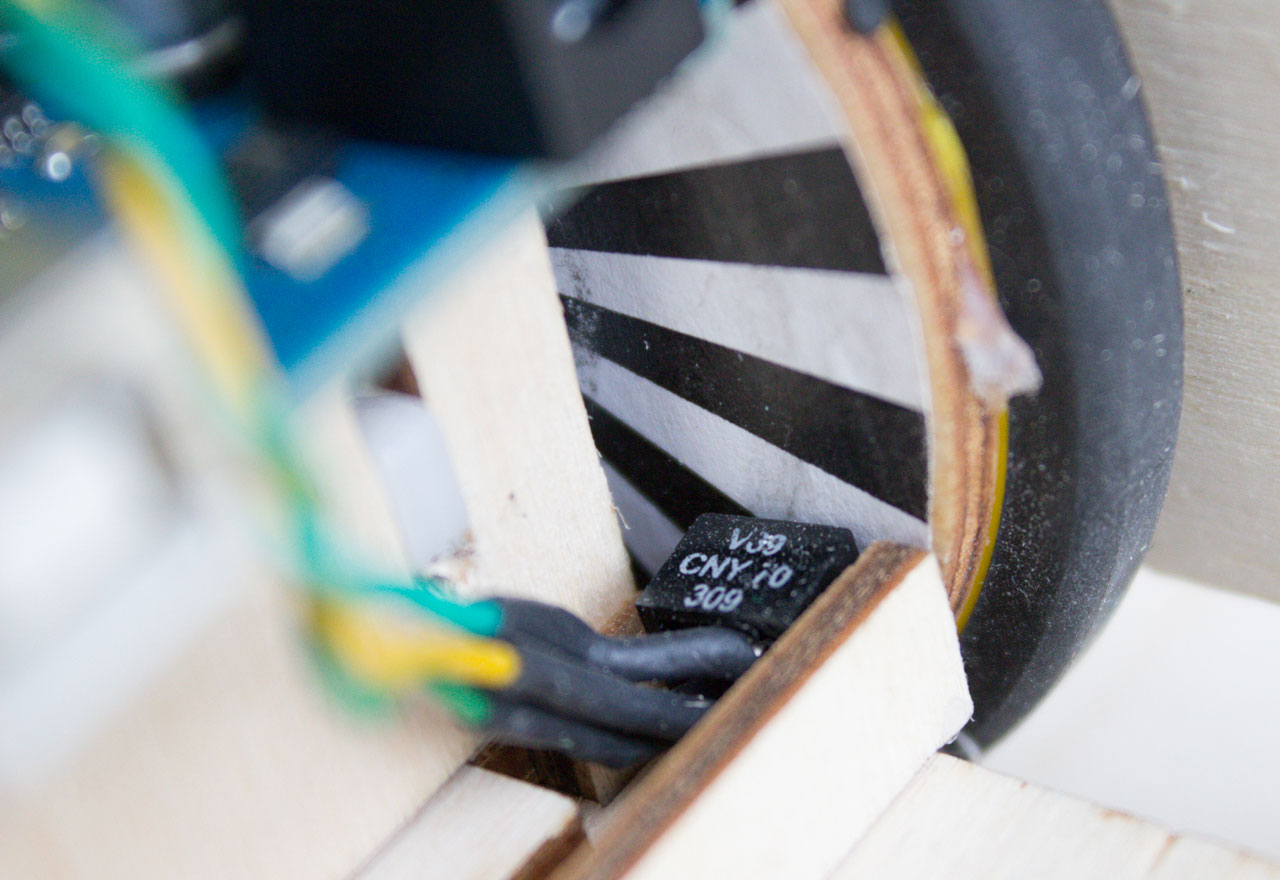
\includegraphics[scale=0.10]{./imagens/diy-docs-10.jpg}
  \caption[ ]{Visão da CNY70 mostrando a proximidade com a roda }
  \label{fig:cny70 no cubetto perto}
\end{figure}

Agora você pode colocar as rodas sobre os motores e, se você utilizou as rodas da Solarbotics, pode aparafusá-las com o parafuso fornecido, mas não aperte muito, ok?

Cole três das quatro ‘paredes' do Cubetto, as partes 5, 7 e 8. Vamos deixar a parte de trás removível, caso queiramos modificar algo mais para a frente.

Pegue o suporte das baterias e solde os cabos preto e vermelho a outros dois conectores fêmea. Os conectores no Módulo serão ligados ao Vin e ao aterramento. Sugerimos a instalação de uma chave (interruptor) que interrompa o fio vermelho.

\begin{figure}[h] % Poderia ser \begin{figure}[posicionamento], onde o posicionamento pode ser h - no local do texto onde foi  o comando, t - no topo da pagina atual ou b - no final da pagina de trabalho.
  \centering
  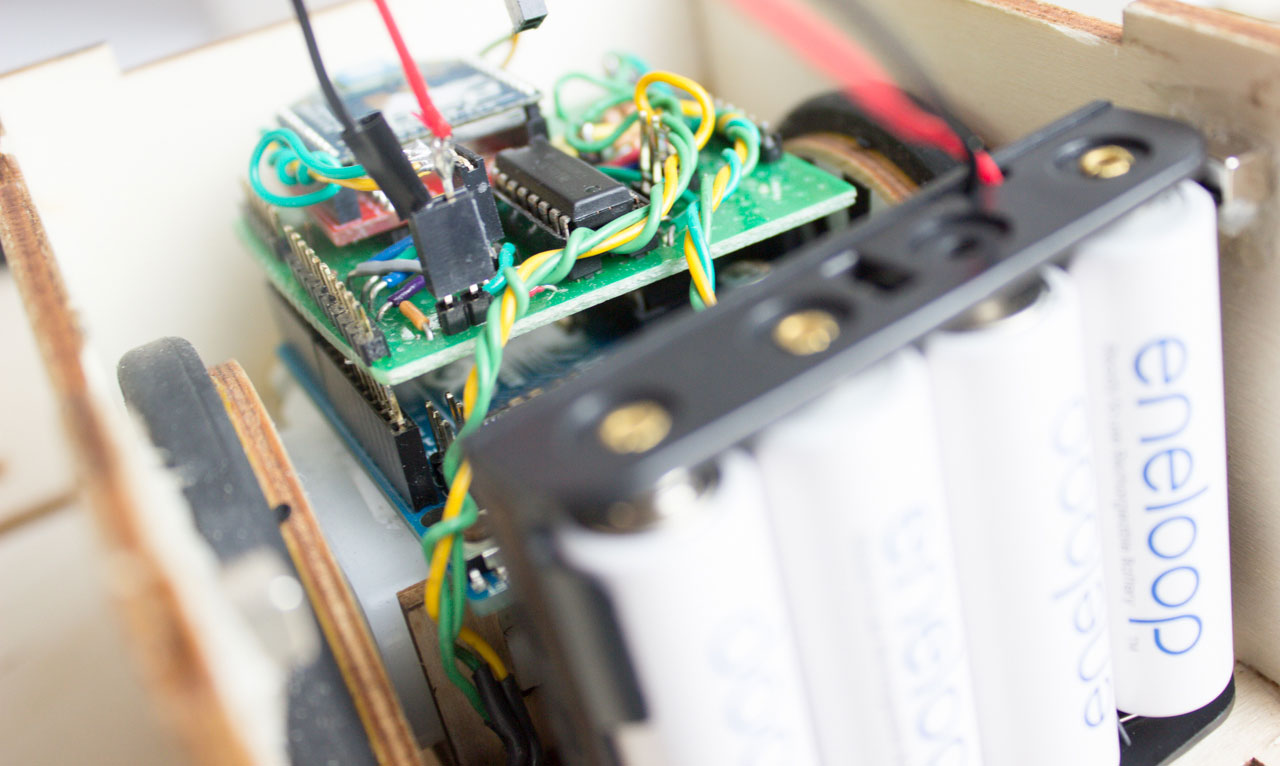
\includegraphics[scale=0.10]{./imagens/diy-docs-13.jpg}
  \caption[ ]{Imagem do suporte de bateria no Cubetto }
  \label{fig:bateria no cubetto}
\end{figure}

Agora você pode colocar o conjunto Arduino + Módulo Wireless por cima dos motores, plugar todos os conectores na placa e no Módulo e você terminou de fazer o Cubetto!



\subsection{Arduino}


As instruções estão contidas nos próprios comentários dentro do código de programação (Sketch) na conta do Github \textit{https://github.com/primo-io/}, repositório \textit{CubettoPlayset-Sketches}.


\end{document}